%%%%%%%%%%%%%%%%%%%%%%%%%%%%%%%%%%%%%%%%%%%%%%%%%%%%%%%%%%%%%%%%%%%%%%%%%%%%%%
%
% Space Warps System Paper
%
%%%%%%%%%%%%%%%%%%%%%%%%%%%%%%%%%%%%%%%%%%%%%%%%%%%%%%%%%%%%%%%%%%%%%%%%%%%%%%

\documentclass[useAMS,usenatbib,a4paper]{mn2e}
%% letterpaper
%% a4paper

\voffset=-0.6in

% Packages:
\input psfig.sty
\usepackage{xspace}
\usepackage{graphicx}
\usepackage{amssymb}
\usepackage{amsmath}

% Macros:
% JOURNALS
\newcommand{\apj}{ApJ}
\newcommand{\apjl}{ApJL}
\newcommand{\apjs}{ApJS}
\newcommand{\mnras}{MNRAS}
\newcommand{\apss}{Ap \& SS}
\newcommand{\aap}{A\&A}
\newcommand{\aj}{AJ}
\newcommand{\prd}{Phys. Rev. D}
\newcommand{\nat}{Nature}
\newcommand{\araa}{ARA\&A}
\newcommand{\jgr}{J. Geophys. Res.}
\newcommand{\pasp}{PASP}

% MISC
\newcommand{\etal}{et~al.~}
\newcommand{\eg}{{\it e.g.\ }}
\newcommand{\ie}{{\it i.e.\ }}
\newcommand{\etc}{{\it etc.\ }}

\newcommand{\be}{\begin{equation}}
\newcommand{\ee}{\end{equation}}
\newcommand{\bea}{\begin{eqnarray}}
\newcommand{\eea}{\end{eqnarray}}


% CROSS-REFERENCING
\def\Sref#1{Section~\ref{#1}\xspace}
\def\Fref#1{Figure~\ref{#1}\xspace}
\def\Tref#1{Table~\ref{#1}\xspace}
\def\Eref#1{Equation~\ref{#1}\xspace}
\def\Aref#1{Appendix~\ref{#1}\xspace}

% UNITS
\newcommand{\kms}{\ifmmode  \,\rm km\,s^{-1} \else $\,\rm km\,s^{-1}  $ \fi }
\newcommand{\kpc}{\ifmmode  {\rm kpc}  \else ${\rm  kpc}$ \fi  }  
\newcommand{\pc}{\ifmmode  {\rm pc}  \else ${\rm pc}$ \fi  }  
\newcommand{\Msun}{\ifmmode {\rm M_{\odot}} \else ${\rm M_{\odot}}$ \fi} 
\newcommand{\Zsun}{\ifmmode {\rm Z_{\odot}} \else ${\rm Z_{\odot}}$ \fi} 
\newcommand{\yr}{\ifmmode yr^{-1} \else $yr^{-1}$ \fi} 
\newcommand{\hMsun}{\ifmmode h^{-1}\,\rm M_{\odot} \else $h^{-1}\,\rm M_{\odot}$ \fi}

% COSMOLOGY
\newcommand{\LCDM}{$\Lambda{\rm CDM}$}
\newcommand{\MS}{Millennium Simulation\xspace}

% LENSING
\def\zd{z_{\rm d}}
\def\zs{z_{\rm s}}
\def\Dd{D_{\rm d}}
\def\Ds{D_{\rm s}}
\def\Dt{D_{\Delta t}}
\def\Dds{D_{\rm ds}}
\def\Sigmacrit{\Sigma_{\rm crit}}
\def\REin{R_{\rm Ein}}
\def\MEin{M_{\rm Ein}}

% SOFTWARE/HARDWARE
\def\sw{{\small\sc Space\,Warps}\xspace}
\def\SW{{\sc Space\,Warps}\xspace}
\def\Talk{{\small\sc Talk}\xspace}
\def\Letters{{\small\sc Letters}\xspace}
\def\Letter{{\small\sc Letter}\xspace}
\def\Dashboard{{\small\sc Dashboard}\xspace}
\def\cfhtls{{\it CFHTLS}\xspace}
\def\python{{\sc python}\xspace}

% TABLES:
\newcommand\nodata{ ~$\cdots$~ }%

% PROBABILITY THEORY
\def\pr{{\rm Pr}}
\def\data{{\mathbf{d}}}
\def\datap{{\mathbf{d}^{\rm p}}}
\def\datai{d_i}
\def\datapi{d^{\rm p}_i}
\def\LENS{{\rm LENS}}
\def\saidLENS{{\rm ``LENS"}}
\def\NOT{{\rm NOT}}
\def\saidNOT{{\rm ``NOT"}}

% AGENT BUREAUCRACY
\def\effort{N_{\rm C}}
\def\experience{N_{\rm T}}
\def\skill{\langle I \rangle}
\def\contribution{$\sum_k \skill_k$}
\def\information{\delta I}

% COMMENTING
\usepackage[usenames]{color}
\newcommand{\question}[2]{\textcolor{red}{\bf Question from #1: #2}}
\newcommand{\flag}[2]{\textcolor{blue}{\bf Comment from #1: #2}}
\newcommand{\new}[1]{{\bf #1}}

% RESULTS
\def\Ncollaboration{XXX}

\def\oxford{Dept.\ of Physics, University of Oxford, Keble Road, Oxford, OX1 3RH, UK}
\def\oxfordeng{Dept.\ of Engineering Science, University of Oxford, Parks Road, Oxford, OX1 3PJ, UK}
\def\kipac{Kavli Institute for Particle Astrophysics and Cosmology, Stanford University, 452 Lomita Mall, Stanford, CA 94035, USA}
\def\ipmu{Kavli IPMU (WPI), University of Tokyo, 5-1-5 Kashiwanoha, Kashiwa 277-8583, Japan}
\def\zooniverse{Zooniverse, c/o Astrophysics Department, University of Oxford, Oxford OX1 3RH, UK}
\def\adler{Adler Planetarium, Chicago, IL, USA}
\def\lausanne{EPFL, Lausanne, Switzerland}
\def\zurich{Department of Physics, University of Zurich, Switzerland}
\def\paris{Institut d’Astrophysique de Paris, UMR7095 CNRS – Universit\'e Pierre et Marie Curie, 98bis bd Arago, 75014 Paris, France}
\def\icg{Institute of Cosmology and Gravitation, University of Portsmouth, Dennis Sciama Building, Portsmouth P01 3FX, UK}

\def\pjmemail{\tt pjm@slac.stanford.edu}
\def\amemail{\tt anupreeta.more@ipmu.jp}


%%%%%%%%%%%%%%%%%%%%%%%%%%%%%%%%%%%%%%%%%%%%%%%%%%%%%%%%%%%%%%%%%%%%%%%%%%%%%%

\title[\sw]
{\SW: Crowd-sourcing the Discovery of Gravitational Lenses}
    
\author[Marshall et al.]{%
  % The \SW Collaboration includes:

% Principal Investigators (opt-out):
   \newauthor{%
    Philip~J.~Marshall,$^{1,2}$\thanks{\pjmemail}
    Aprajita~Verma,$^{2}$
    Anupreeta~More,$^{3}$
    Christopher~P.~Davis,$^{1}$
    }
    \newauthor{%
    Surhud~More,$^{3}$
    Amit~Kapadia,$^{4}$
    Michael~Parrish,$^{4}$
    Chris~Snyder,$^{4}$
    }
   \newauthor{%
    Julianne~Wilcox,$^{5}$
    Elisabeth~Baeten,$^{5}$
    Christine~Macmillan,$^{5}$
    Claude~Cornen,$^{5}$
    }
   \newauthor{%
    Michael~Baumer,$^{1}$
    Edwin~Simpson,$^{6}$
    Chris~J.~Lintott,$^{2}$
    David~Miller,$^{4}$
    }
   \newauthor{%
    Edward~Paget,$^{4}$
    Robert~Simpson,$^{2}$
    Arfon~M.~Smith,$^{4}$
    Rafael~K\"ung,$^{7}$
    }
   \newauthor{%
    Prasenjit~Saha,$^{7}$
    Thomas~E.~Collett$^{8}$
    }
 %
\medskip\\
$^1$\kipac\\
$^2$\oxford\\
$^3$\ipmu\\
$^4$\adler\\
$^5$\zooniverse\\
$^6$\oxfordeng\\
$^7$\zurich\\
$^8$\icg\\

}

%%%%%%%%%%%%%%%%%%%%%%%%%%%%%%%%%%%%%%%%%%%%%%%%%%%%%%%%%%%%%%%%%%%%%%%%%%%%%%

\begin{document}
             
\date{to be submitted to MNRAS}
\pagerange{\pageref{firstpage}--\pageref{lastpage}}\pubyear{2014}

\maketitle           

\label{firstpage}

%%%%%%%%%%%%%%%%%%%%%%%%%%%%%%%%%%%%%%%%%%%%%%%%%%%%%%%%%%%%%%%%%%%%%%%%%%%%%%

\begin{abstract} 

\sw is a web-based service that enables the discovery of strong gravitational
lenses in wide-field imaging surveys by large numbers of people. Carefully
produced color composite images are displayed to volunteers via a
classification interface which records their estimates of the positions of
candidate lensed features. Simulated lenses, and expert-classified non-lenses,
are inserted into the image stream at random intervals; this training set is
used to give the volunteers feedback on their performance, and to estimate a
dynamically-updated probability for any given image to contain a lens. Low
probability systems are retired from the site periodically, concentrating the
sample towards a set of candidates; this ``stage 1'' set is then re-classified
by the volunteers in a second  refinement stage. Analyzing the classification
of the training set, we predict that the first stage alone should yield a
sample that is C\% complete, while leading to the rejection of R\% of the
initial target sample. Having divided the 150 square degree CFHTLS imaging
survey into 430000 overlapping 70 by 70 arcminute tiles and displayed them on
the site, we were joined by 33000 volunteers who contributed X million image
classifications over the course of N months. The sample was reduced to 3500
stage 1 candidates; these were then refined to yield a sample of 1400
candidates rankable by their stage 2 probability. We expect this sample to be
X\% complete and Y\% pure at a threshold of 95\% classification probability.
We find that, on average, and given the assumptions we make in our analysis,
we need 9 classifications per image during the first stage, X in the second.
We estimate the mean information contributed per person to be X bits, over a
session lasting, on average, N classifications per volunteer, and present the
highly skewed distributions of these quantities. We comment on the scalability
of the \sw system to the wide field survey era, and its potential to operate
beyond its design as a supervised classification system. 

\end{abstract}

% Full list of options at http://www.journals.uchicago.edu/ApJ/instruct.key.html

\begin{keywords}
  gravitational lensing   --
  methods: statistical    --
  methods: citizen science
\end{keywords}

\setcounter{footnote}{1}

%%%%%%%%%%%%%%%%%%%%%%%%%%%%%%%%%%%%%%%%%%%%%%%%%%%%%%%%%%%%%%%%%%%%%%%%%%%%%%

\section{Introduction}
\label{sec:intro}

% Scientific motivation. Applications of lenses: group-scale arcs,
% galaxy-galaxy lenses, lensed quasars. 

Strong gravitational lensing -- the formation of multiple, magnified images of
background objects due to the deflection of light by  massive foreground
objects -- is a very powerful astrophysical tool, enabling a wide range of
science projects. The image separations and distortions provide information
about the mass distribution in the lens \citep[e.g.][]{AugerEtal2010,
SonnenfeldEtal2012,SonnenfeldEtal2013}, including on sub-galactic scales
\citep[e.g.][]{Dalal+Kochanek2002,VegettiEtal2010,HezavehEtal2013}. Any
strong lens can provide magnification of a factor of 10 or more, providing a
deeper, higher resolution view of the distant universe through these ``cosmic
telescopes'' \citep[e.g.][]{StarkEtal2008,NewtonEtal2011}. Lensed quasars enable
cosmography via the time delays between the multiple images' lightcurves
\citep[e.g.][]{TewesEtal2013,SuyuEtal2013}, and study of the accretion disk itself
through the microlensing effect \citep[e.g.][]{PoindexterEtal2008}. All of these
science projects would benefit from being able to draw from a larger sample of
lenses.

In the last decade the numbers of detections of these rare cosmic alignments
has increased by an order of magnitude, thanks to wide field surveys such as
CLASS \citep[e.g.]{BrowneEtal2003}, SDSS \citep[e.g.][]
{BoltonEtal2006,AugerEtal2010b,TreuEtal2011,InadaEtal2012}, CFHTLS
\citep[e.g.][]{MoreEtal2012,GavazziEtal2014}, Herschel
\citep[][]{NegrelloEtal2014} and SPT \citep[e.g.][]{VieiraEtal2013}, among
others.  As the number of known lenses has increased, new types have been
discovered, leading to entirely new investigations. Compound lenses
\citep{GavazziEtal2008,CollettEtal2012} and lensed supernovae
\citep{QuimbyEtal2014} are good examples of this. 

% Problem of rarity. Imaging surveys. Problem of purity/false positives.
% Review of progress to date. Methods in SL2S, SQLS. Contrast with SLACS. 

Because they are rare, strong lenses are expensive to find. The most efficient
searches to date have made use of relatively clean signals such as the
presence of emission or absorption features at two distinct redshifts in the
same optical spectrum \citep[e.g.][]{BoltonEtal2004}, or the strong
``magnification bias'' towards detecting strongly-lensed sources in the sub-mm
waveband \citep[e.g.][]{NegrelloEtal2010}. Such searches have to be efficient,
because they require expensive high resolution imaging follow-up; consequently
they have so far produced yields in the tens to hundreds. An alternative approach
is to search images of sufficiently high resolution and color contrast, and
confirm the systems as gravitational lenses by modeling the survey data
themselves \citep[][]{MarshallEtal2009}. Several square degrees of HST images
have been searched, yielding several tens of galaxy-scale lenses
\citep[e.g.][]{MoustakasEtal2007,FaureEtal2008,Jackson2008,MoreEtal2012,
PawaseEtal2014}.
Similarly, searches of over a hundred square degrees of CFHT Legacy Survey
ground-based imaging, also with sub-arcsecond image quality, have revealed a
smaller number of wider image separation group-scale systems
\citep[e.g.][]{CabanacEtal2007,MoreEtal2012}. Detecting galaxy-scale lenses from
the ground is hard, but feasible albeit lower efficiency and requiring HST or
spectroscopic follow-up to confirm the candidates as lenses
\citep[e.g.][]{GavazziEtal2014}.

% Scaling to wide field era. Automated methods: problems. Need for good
% training sets. Need for quality control: always present.

How can we scale these lens searches up to imaging surveys covering a hundred
times the sky area, such as the almost-all sky surveys planned with LSST and
Euclid, while reducing our dependence on expensive follow-up confirmation
observations? There are two approaches to detecting lenses in imaging surveys.
The first one is robotic: automated analysis of object catalogs and/or the
survey images. The candidate samples produced by these methods have, to date,
not been of high purity  \citep[see
e.g.][]{MarshallEtal2009,MoreEtal2012,GavazziEtal2014}, with visual inspection by
teams of humans still required to narrow down the robotically-generated
samples. In this approach, the image data may or may not be explicitly
modelled by the robots as if it contained a gravitational lens, but the visual
inspection can be thought of as a ``mental modeling'' step. Systems classified
by an inspector to be good lens candidates are deemed as such because the
features in the image can be explained by a model of what gravitational lenses
do contained in the inspector's brain. The second approach simply cuts out the
robot middleman: \citet{FaureEtal2008,Jackson2008} and \citet{PawaseEtal2014}
all performed entirely visual searches for lenses in HST imaging.

Visual image inspection seems, at present, unavoidable at some level when
seraching for gravitational lenses. The technique has some drawbacks, however.
First is that humans are only humans, and they make mistakes. The solution to
this is to operate in teams, providing multiple classifications of the same
images in order to catch errors and correct them. Second, and relatedly, is
that humans get tired. With a well-designed classification interface, a human
might be able to inspect images at a rate of one astronomical object per
second (provided the majority are indeed uninteresting). At $10^4$ massive
galaxies, and 10 lenses, per square degree, visual lens searches in good
quality imaging data are limited to a few square degrees per inspector per
day. Scaling to thousands of square degrees therefore means either robotically
reducing the number of targets for inspection, or increasing the number of
inspectors, or both. 

For example, a $10^4$ square degree survey containing $10^8$
photometrically-selected massive galaxies and $10^5$ lenses could only be
searched by 10 inspectors at a mean rate of 1 galaxy per second and 10
inspections per galaxy in about 14 years. Reducing the inspection time by a
factor of 400 to two weeks would require a robot to reduce the target sample
to 25 per square degree. However, at this point the required purity, 40\%,
would very likely require the average classification time per object to be
more like 10 seconds per object. Hiring 10 inspectors to assess complex images
full time full time for five months may not be the most cost-effective or
reliable strategy. Alternatively, a team of $10^6$ inspectors could, in
principle, make the required $10^9$ image classifications, $10^3$ each, in a
few weeks; robotically reducing the target list would lead to a proportional
decrease in the required team size.

Systematic detection of rare astronomical objects by such ``crowd-sourced''
visual inspection has recently been achieved by the online citizen science
project PlanetHunters \citep{SchwambEtal2012}. PlanetHunters was designed to
enable the discovery of transiting exoplanets in data taken by the Kepler
satellite; a community of N inspectors from the general public found, after
each undergoing a small amount of training, N new exoplanet candidates by
visual inspection of the Kepler lightcurves that were presented in a custom
web-based classification interface. The older Galaxy Zoo morphological
classification project \citep{LintottEtal2008} has also enabled the discovery
of rare objects, via its flexible inspection interface and discussion forum
\citep{LintottEtal2009}. Indeed, several of us (AV,EB,CC,TJ,CM,LW) were active
in an informal Galaxy Zoo gravitational lens search, an experience which led
to the present hypothesis that a systematic online visual lens search could be
successful. 

In this paper, we describe the \sw website, an online system that enables 
crowd-sourced gravitational lens detection by inviting volunteers to classify
astronomical survey images as containing lens candidates or not.  In a
companion paper we will present the new gravitational lenses discovered in our
first experimental lens search, and begin to investigate the differences
between lens detections made in \sw and those made with automated techniques.
Here though, we try to answer the following questions:

\begin{itemize}

\item How reliably can we find gravitational lenses using the \sw
system? What is the completeness of the sample produced?

\item How noisy is the system? What is the purity of the sample
produced?

\item How quickly can lenses be detected, and non-lenses be rejected?
How many classifications, and so how many volunteers are needed per target?

\item What can we learn about the scalability of the crowd-sourcing approach?

\end{itemize}

This paper is organised as follows.  In \Sref{sec:design} we introduce the \sw
classification interface and the volunteers who make up the \sw
collaboration,  explain how we use training images, and describe our two stage
candidate selection strategy. We then briefly introduce, in \Sref{sec:data}
the particular dataset used in the first experimental tests of the \sw system,
and how we prepared the images prior to displaying them in the web interface.
In \Sref{sec:swap} we describe our methodology for interpreting the
classifications made by the volunteers, and then present the results of system
performance tests  made on the training images in \Sref{sec:results}. % In
this section, we also investigate the properties of the crowd, to % understand
where the information is coming from. We discuss the implications of our
results for future lens searches in \Sref{sec:discuss} and draw conclusions in
\Sref{sec:conclude}.

% \section{Introduction}
% \label{sec:intro}
% \section{Experiment Design}
% \label{sec:design}
% \subsection{Training}
% \label{sec:design:training}
% \subsection{Stage 1: Initial Classification}
% \label{sec:design:stage1}
% \subsection{Stage 2: Refinement}
% \label{sec:design:stage2}
% \section{Data}
% \label{sec:data}
% \subsection{The CFHT Legacy Survey}
% \label{sec:data:CFHTLS}
% \subsection{Image Presentation}
% \label{sec:data:display}
% \section{Classification Analysis}
% \label{sec:swap}
% \section{Results}
% \label{sec:results}
% \subsection{Crowd Properties}
% \label{sec:results:crowd}
% \subsection{Sample completeness and purity}
% \label{sec:results:sample}
% \section{Discussion}
% \label{sec:discuss}
% \section{Conclusions}
% \label{sec:conclude}

%%%%%%%%%%%%%%%%%%%%%%%%%%%%%%%%%%%%%%%%%%%%%%%%%%%%%%%%%%%%%%%%%%%%%%%%%%%%%%

\section{Experiment Design}
\label{sec:design}

The basic steps of a visual search for gravitational lenses are: 1) prepare
images, 2) display them to an inspector, 3) record the inspector's
classification of each image (as, for example, containing a lens candidate or
not) and 4) analyzing those classifications (and all others) in order to
produce a final candidate list. We describe step 1 in \Sref{sec:data} and step
4 in \Sref{sec:swap}. In this section we take a volunteer's eye view and
begin by describing the \sw classification interface, the crowd of volunteers,
and the interactions between the two.

%%%%%%%%%%%%%%%%%%%%%%%%%%%%%%%%%%%%%%%
\begin{figure*}
\centering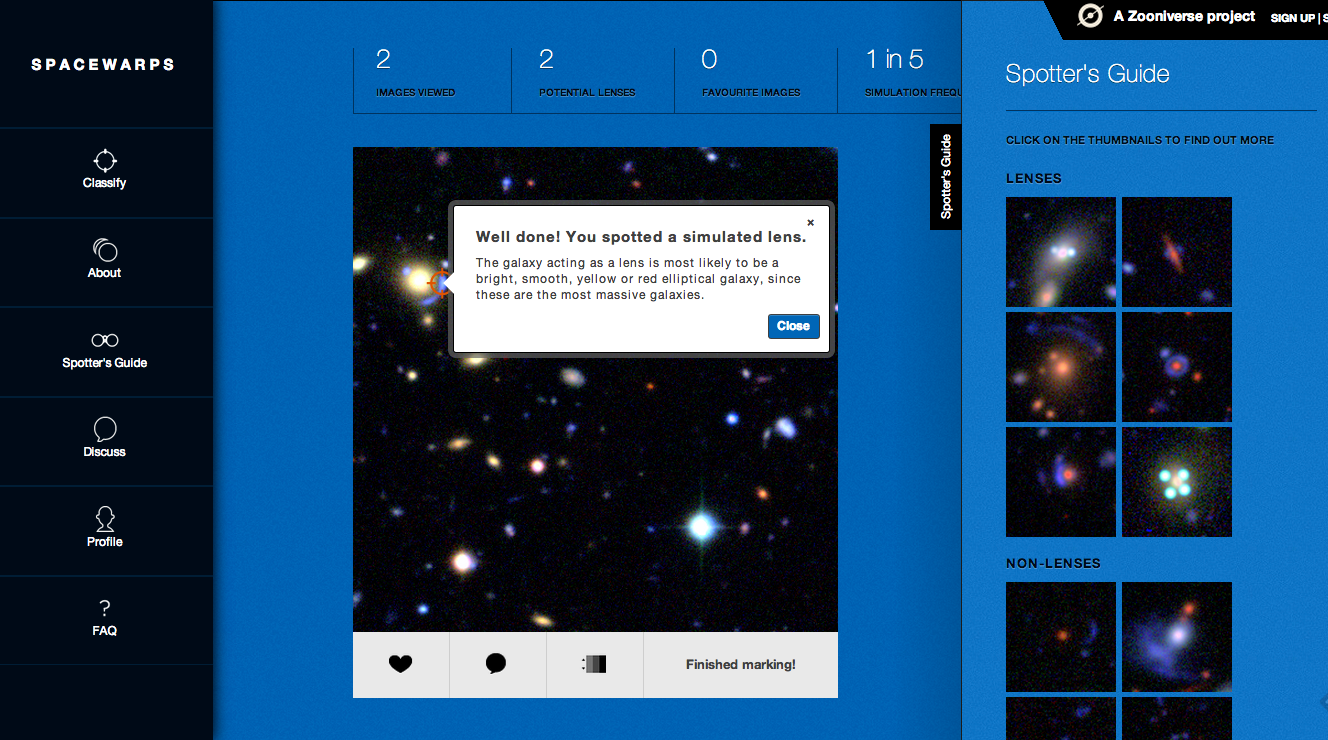
\includegraphics[width=0.9\linewidth]{sw-system-figs/sw-screengrab-marker+feedback.png}
\caption{Screenshot of the \sw classification interface.}
\label{fig:screenshot}
\end{figure*}
%%%%%%%%%%%%%%%%%%%%%%%%%%%%%%%%%%%%%%%

% % % % % % % % % % % % % % % % % % % % % % % % % % % % % % % % % % % % % % % 

\subsection{Classification Interface}
\label{sec:design:interface}

A screenshot of the \sw classification interface (CI) is shown in
\Fref{fig:screenshot}. The CI is the centrepiece of the \sw website,
\texttt{http://spacewarps.org}; the web application is written in
coffeescript, css and html and follows the general design of others written by
the Zooniverse team.\footnote{The \sw web application code is open source and
can be accessed from \texttt{https://github.com/zooniverse/Lens-Zoo}}  The
focus of the CI is a large display of the current pre-prepared PNG image of
the ``subject'' being inspected.   When the image is clicked on by the
volunteer, a marker symbol appears where the pointer was. Several markers can
be placed.  The next image moves rapidly in from a queue formed at the right
hand side of the screen when the ``Finished marking'' button is pressed. At
the same time, the positions of the markers are written out to the
classification database, in an entry that also stores the ID of the subject,
the username (or IP address) of the volunteer, a timestamp and some other
metadata. 

Gravitational lenses are rare: typically, most of the images will not contain
a lens candidate, and these need to be quickly rejected by the inspector. The
queue allows several images to be pre-loaded while the volunteer is
classifying the current subject, and the rapid movement is designed to
encourage volunteers to classify rapidly.

For the more interesting subjects, the CI offers two features that  enable
further investigation of the subjects. First is the ``Quick Dashboard'' (QD) a
more advanced image viewer. This allows the viewer to compare three different
contrast and color balance settings, to help bring out subtle features, and to
zoom in on interesting regions of the image to assess small features. Markers
can be placed in the Quick Dashboard just the same as in the main CI image
viewer. The second is a link to that subject's page in the project discussion
forum, \texttt{http://talk.spacewarps.org}. Here, volunteers can discuss the
features they have seen either before they submit their classification, or
after, if they ``favorite'' the subject. There is no ``back'' button: each
volunteer may only classify a given subject once. However, the presence of an
option to see what others think about any given subject before submitting your
own classification means that the classifications may not be  strictly
independent; the advantage of this system is that volunteers can learn from
others what constitutes a good lens candidate. In practice, we might expect
this to be a relatively unimportant educational resource, given the explicit
training we provide for the volunteers, which we describe in the next section.


% % % % % % % % % % % % % % % % % % % % % % % % % % % % % % % % % % % % % % % 

\subsection{Training}
\label{sec:design:training}

Gravitational lenses are unfamiliar objects to volunteers who are new
to the site. New volunteers need to learn what lenses look like as quickly as
possible, so that they can contribute informative classifications. They also
need to learn what lenses do not look like, in order to reduce the false
positive detection rate. There are three primary mechanisms in the \sw system
for teaching the volunteers what to look for. These are, in the order in which
they are encountered, an inline tutorial, instant feedback,
and a ``Spotter's Guide.''

\subsubsection{Inline Tutorial}

New volunteers are welcomed to the site with a very short tutorial, in which
the task is introduced, a typical image containing a simulated lens is
displayed, and the marking procedure walked through, using pop-up message
boxes. Subsequent images gradually introduce the more advanced
features of the classification interface (the QD and Talk buttons), also using
pop-up messages. The tutorial was purposely kept as short as possible so as to
provide the minimal barrier to entry.

\subsubsection{Training Subjects and Instant Feedback}

The second image viewed after the initial tutorial image is already a survey
image, in order to get the volunteers engaged in the real task as quickly as
possible. Training continues beyond the first image tutorial through
``training subjects'' inserted randomly into the stream.  These training
subjects are either simulated lenses (known as ``sims''), or survey images
that were expert-classified (by AV, AM and PM) and found not to contain any
lens candidates (these images are known as ``duds''). The tutorial explains
that the volunteers  will be shown such training images. They are also
informed that they will receive instant feedback about their performance after
classifying (blind) any of these training subjects. Indeed, after a volunteer
finishes marking a training subject and hits ``Finished marking,'' a pop-up
message is generated, containing either positive feedback for a successful
classification (for example, ``Well done! You spotted a simulated lens,'' as
in \Fref{fig:screenshot}) or negative feedback for an unsuccessful one (for
example, ``There is no gravitational lens in this field!'') 


The initial frequency of the training images is set to be two in five;
subjects are drawn randomly from the pool of training images with this
frequency. The pool contains equal numbers of sims and duds, and the draw is
made without replacement (for that volunteer). As the number of
classifications made by a volunteer increases, this frequency is decreased, to
$2/(5\times2^{(\textrm{int}(N_c/20)+1)/2})$ ($\approx 0.3$ for the second 20
subjects, $0.2$ for the third 20 subjects, and so on).

This training regime means that in the first 60 images viewed, each volunteer
is shown (on average) 9 simulated gravitational lenses, and 9 empty fields. 
This is a much higher rate than the natural one: to try and avoid this leading
to over-optimism among the inspectors (and a resulting high false positive
rate), we display the current ``Simulation Frequency'' on the classification
interface (``1 in 5'' in \Fref{fig:screenshot}) and maintain the consistent
theme in the feedback messages that lenses are rare.


\subsubsection{Spotter's Guide}

The instant feedback provides real-time educational responses to the
volunteers as they start classifying; as well as this dynamic system, \sw
provides a static reference work for volunteers to consult when in doubt about
how to perform the task. This ``Spotter's Guide'' is a set of webpages showing
example lenses, both real and simulated, and also some common false positives,
drawn from the pool of survey images. The non-lenses were identified by three
of us (AV, AM and PM) while inspecting a small set of survey images in order
to define the ``dud'' training images. For easy reference, the lenses are
divided by type (for example, ``lensed galaxies,'' ``lensed quasars'' and
``cluster lenses''), as are the false positives (for example, ``Rings and
Spirals,'' ``Mergers,'' ``Artifacts'' and so on). The example images are
accompanied by explanatory text. The Spotter's Guide is reached via a button
on the left hand side, or the hyperlinked thumbnail images of the ``Quick
Reference'' provided on the right hand side, of the classification interface.

Most of the text of the Spotter's Guide focuses on what lenses do or don't do;
the website ``Science page'' contains a very brief introduction to how
gravitational lenses work, which is fleshed out a little on the ``FAQ'' page. 
This also contains answers to frequently asked questions about the interface
and the task set. 

% % % % % % % % % % % % % % % % % % % % % % % % % % % % % % % % % % % % % % % 

\subsection{Staged Classification}
\label{sec:design:stages}

We now describe briefly the two-stage strategy that was employed in the CFHTLS
project, initial classification (involving the rejection of very large numbers
of non-lenses), and refinement (to further narrow down the sample). The web
application was reconfigured between the two stages, to assist in their
functioning.

\subsubsection{Stage 1: Initial Classification}

The goal of a stage 1 classification is to achieve a high rejection rate,
while maintaining high completeness.  In this mode, therefore, the pre-loading
of images was used to make the sliding in of new subjects happen quickly, to
provide a sense of urgency: initial classification must be done fairly
quickly for the search to be completed within a reasonable time period.  We
expect some trade-off between speed and accuracy, which we return to in the
results section below. Completion of the search requires subjects to be
``retired'' over time, as a result of their being classified. We do this by
analyzing the classifications on a daily basis, as described in
\Sref{sec:swap} below. As subjects are retired, new ones are ingested into
the web app for classification. This means that the discovery of lens
candidates in stage 1 is truly a community effort: to detect a lens candidate,
many non-lenses must first be rejected.

The stage 1 training set was chosen to be quite clear cut, in order to err on
the side of inclusivity, and so ensure high completeness. For the training
duds we selected several hundred images at random, and three of us (AV, AM,
PM) inspected them and discarded anything that could be a lens candidate. The
remainder were ingested into the site.


\subsubsection{Stage 2: Refinement}

At stage 2, the goal is to define a final sample that has both high
completeness and high purity. To this end, a more demanding training set was
defined, where the duds all contain an object identified by one of us (AV, AM
and PM) as a potential false positive. \Fref{fig:training:gallery} shows some
example images from the CFHTLS stage 2 training set. 

\todo{Phil}{Show some example sims and duds...}

We also attempted to encourage discernment by changing the look and feel of
the app, slowing down the arrival of new images, and switching the background
color to bright orange to make it clear that a different task was being set.
The frequency with which training images were shown was fixed at 1 in 3.
Finally, the Spotter's Guide was upgraded to include more detailed discussion
of various possible false positives.


%%%%%%%%%%%%%%%%%%%%%%%%%%%%%%%%%%%%%%%%%%%%%%%%%%%%%%%%%%%%%%%%%%%%%%%%%%%%%%

\section{Data}
\label{sec:data}

Definitions: training subjects and test subjects. Sims and duds.

% % % % % % % % % % % % % % % % % % % % % % % % % % % % % % % % % % % % % % % 

\subsection{The CFHT Legacy Survey}
\label{sec:data:CFHTLS}

Describe survey. Refs. 

Why this one? Good IQ, deep, colorful, homogeneous. Precursor to Stage III and
IV imaging surveys, DES, KIDS, LSST etc. Already searched by robots: enables
comparison of techniques. Lenses not yet found by robots, detectable by
humans? 

Blind search strategy.
Preparation of data: divide survey into overlapping tiles. 


% % % % % % % % % % % % % % % % % % % % % % % % % % % % % % % % % % % % % % % 

\subsection{Image Presentation}
\label{sec:data:display}

Presentation of images. Uniform scales, to build intuition and avoid rescales
due to bright objects. Arcsinh stretch, to bring out low SB features. 
Approximately optimized, how? Examples of images.


%%%%%%%%%%%%%%%%%%%%%%%%%%%%%%%%%%%%%%%%%%%%%%%%%%%%%%%%%%%%%%%%%%%%%%%%%%%%%%

\section{Classification Stages and Analysis}
\label{sec:swap}

In this section we outline our methodology for interpreting the interactions
of the volunteers with the identification interface, and then describe how we
applied this methodology in the two classification stages in the CFHTLS
project.

Each classification made is logged in a database, storing subject IDs,
(anonymous) volunteer IDs, a timestamp and the classification results.  The
{\it kind} of subject -- whether it is a training subject (a  simulated lens
or a known non-lens) or a test subject (an unseen image drawn from the survey)
-- is also recorded. For all subjects, the positions of all Markers are
recorded, in pixel coordinates. For training subjects, we also store the
``classification'' of the subject as a lens, or a non-lens, and also the type
of object present in the image. These types are summarized in
\Tref{tab:objecttypes}.  This classification is used to provide instant
feedback, but is also the basic measurement used in a probabilistic
classification of every subject based on all image views to date.

We perform an online analysis of the classifications,  updating a
probabilistic model of every (anonymous) volunteer's data, and also updating
the lens probability of each subject  (in both the training and test sets), on
a daily basis. This gives us a dynamic estimate of the posterior probability
for  any given  subject being a lens, given all classifications of it to date.
Assigning thresholds in this lens probability then allows us to make good
decisions about whether or not to retire a subject from the system, in order to
focus attention on new images. 

The details of how the lens probabilities are calculated are given in
\Aref{appendix:swap}. In summary:
\begin{itemize}

\item Each volunteer is assigned a simple software agent, characterised by a
confusion matrix. The two independent elements of this matrix are the
probabilities, as estimated by the agent, that the volunteer is going to be 1)
correct when they report that an image contains a lens when it really does
contain a lens, $\pr(\saidLENS|\LENS,T)$, and 2) correct when they report that
an image does not contain a lens when it really doesn't contain a lens,
$\pr(\saidNOT|\LENS,T)$.

\item Each agent updates its confusion matrix elements based on the number of
times its volunteer has been right in each way while classifying subjects from
the training set, accounting for noise early on due to small number
statistics: $T$ is the set of all training images seen to date.

\item Each agent uses its confusion matrices to update, via Bayes' theorem,
the probability of an image from the test set containing a lens,
$\pr(\LENS|C,T)$, when that image is classified by its volunteer. ($C$ is the
set of all classifications made of this subject.)

\end{itemize}

%%%%%%%%%%%%%%%%%%%%%%%%%%%%%%%%%%%%%%%
\begin{figure}
\centering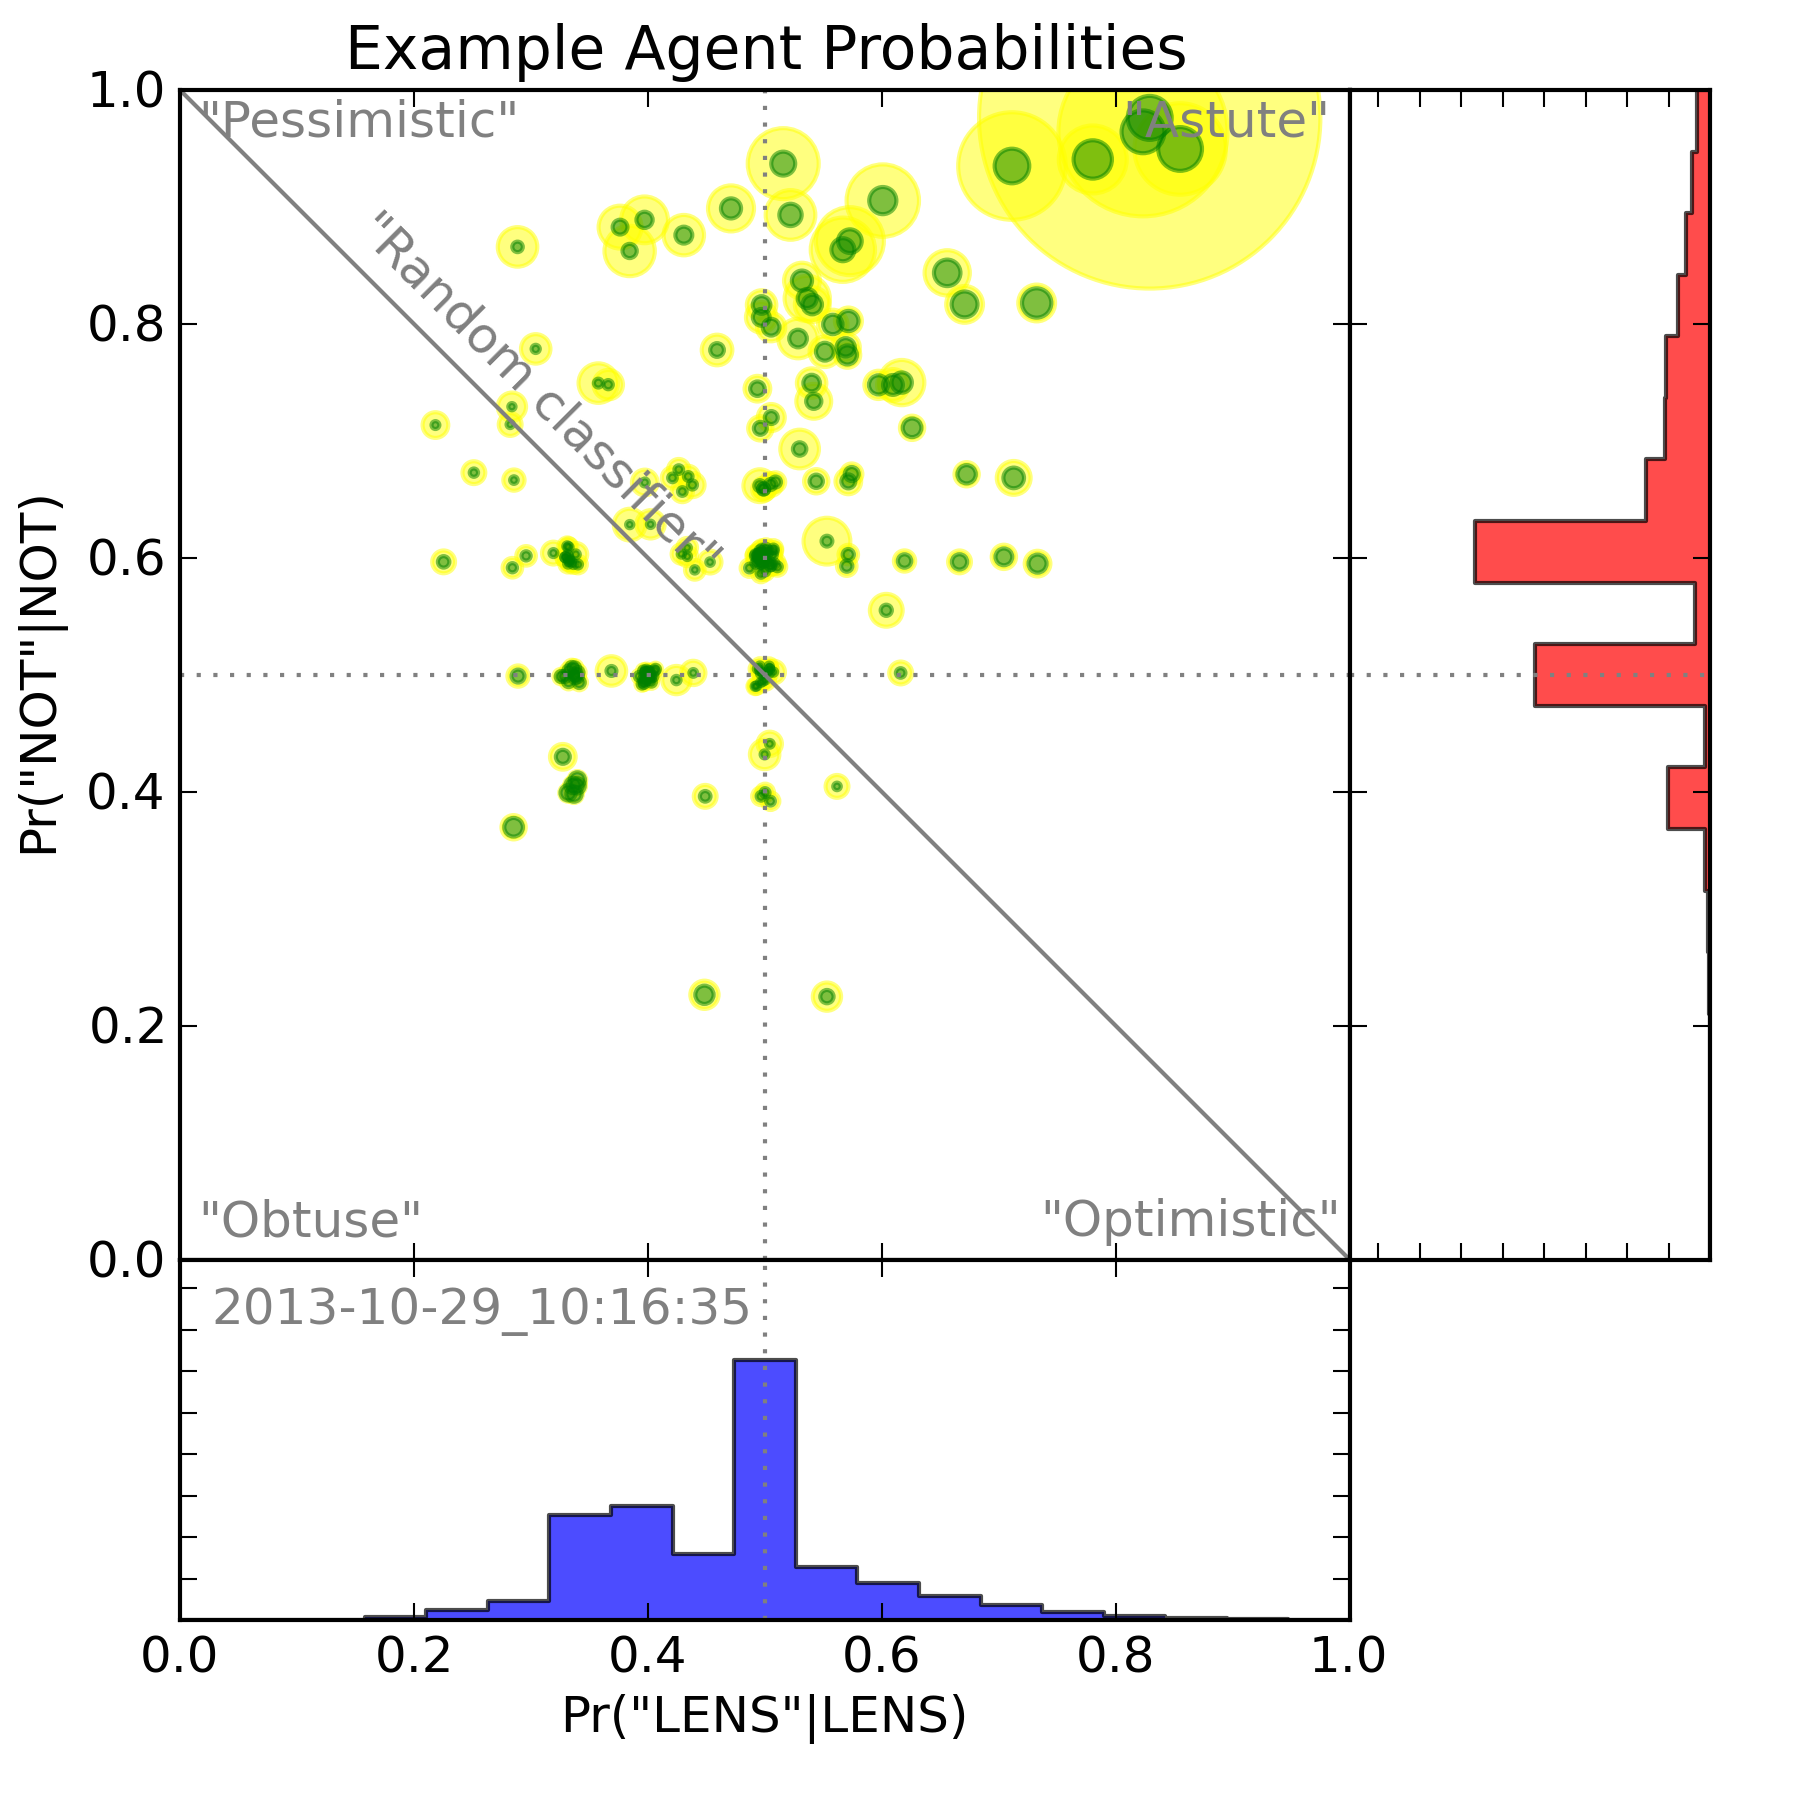
\includegraphics[width=0.9\linewidth]{sw-system-figs/CFHTLS_2013-10-29_10:16:35_probabilities.png}
\caption{Typical \SW Agent confusion matrix elements. At a particular
snapshot, 200 random Agents are shown distributed over the unit plane, with a
tendency to move towards the ``astute'' region in the upper right hand
quadrant as the Agents' volunteers view more images. Yellow point size is
proprtional to the number of images classified; green point size shows
Agent-perceived ``skill.''}
\label{fig:swap:agent-probabilities}
\end{figure}
%%%%%%%%%%%%%%%%%%%%%%%%%%%%%%%%%%%%%%%

%%%%%%%%%%%%%%%%%%%%%%%%%%%%%%%%%%%%%%%
\begin{figure}
\centering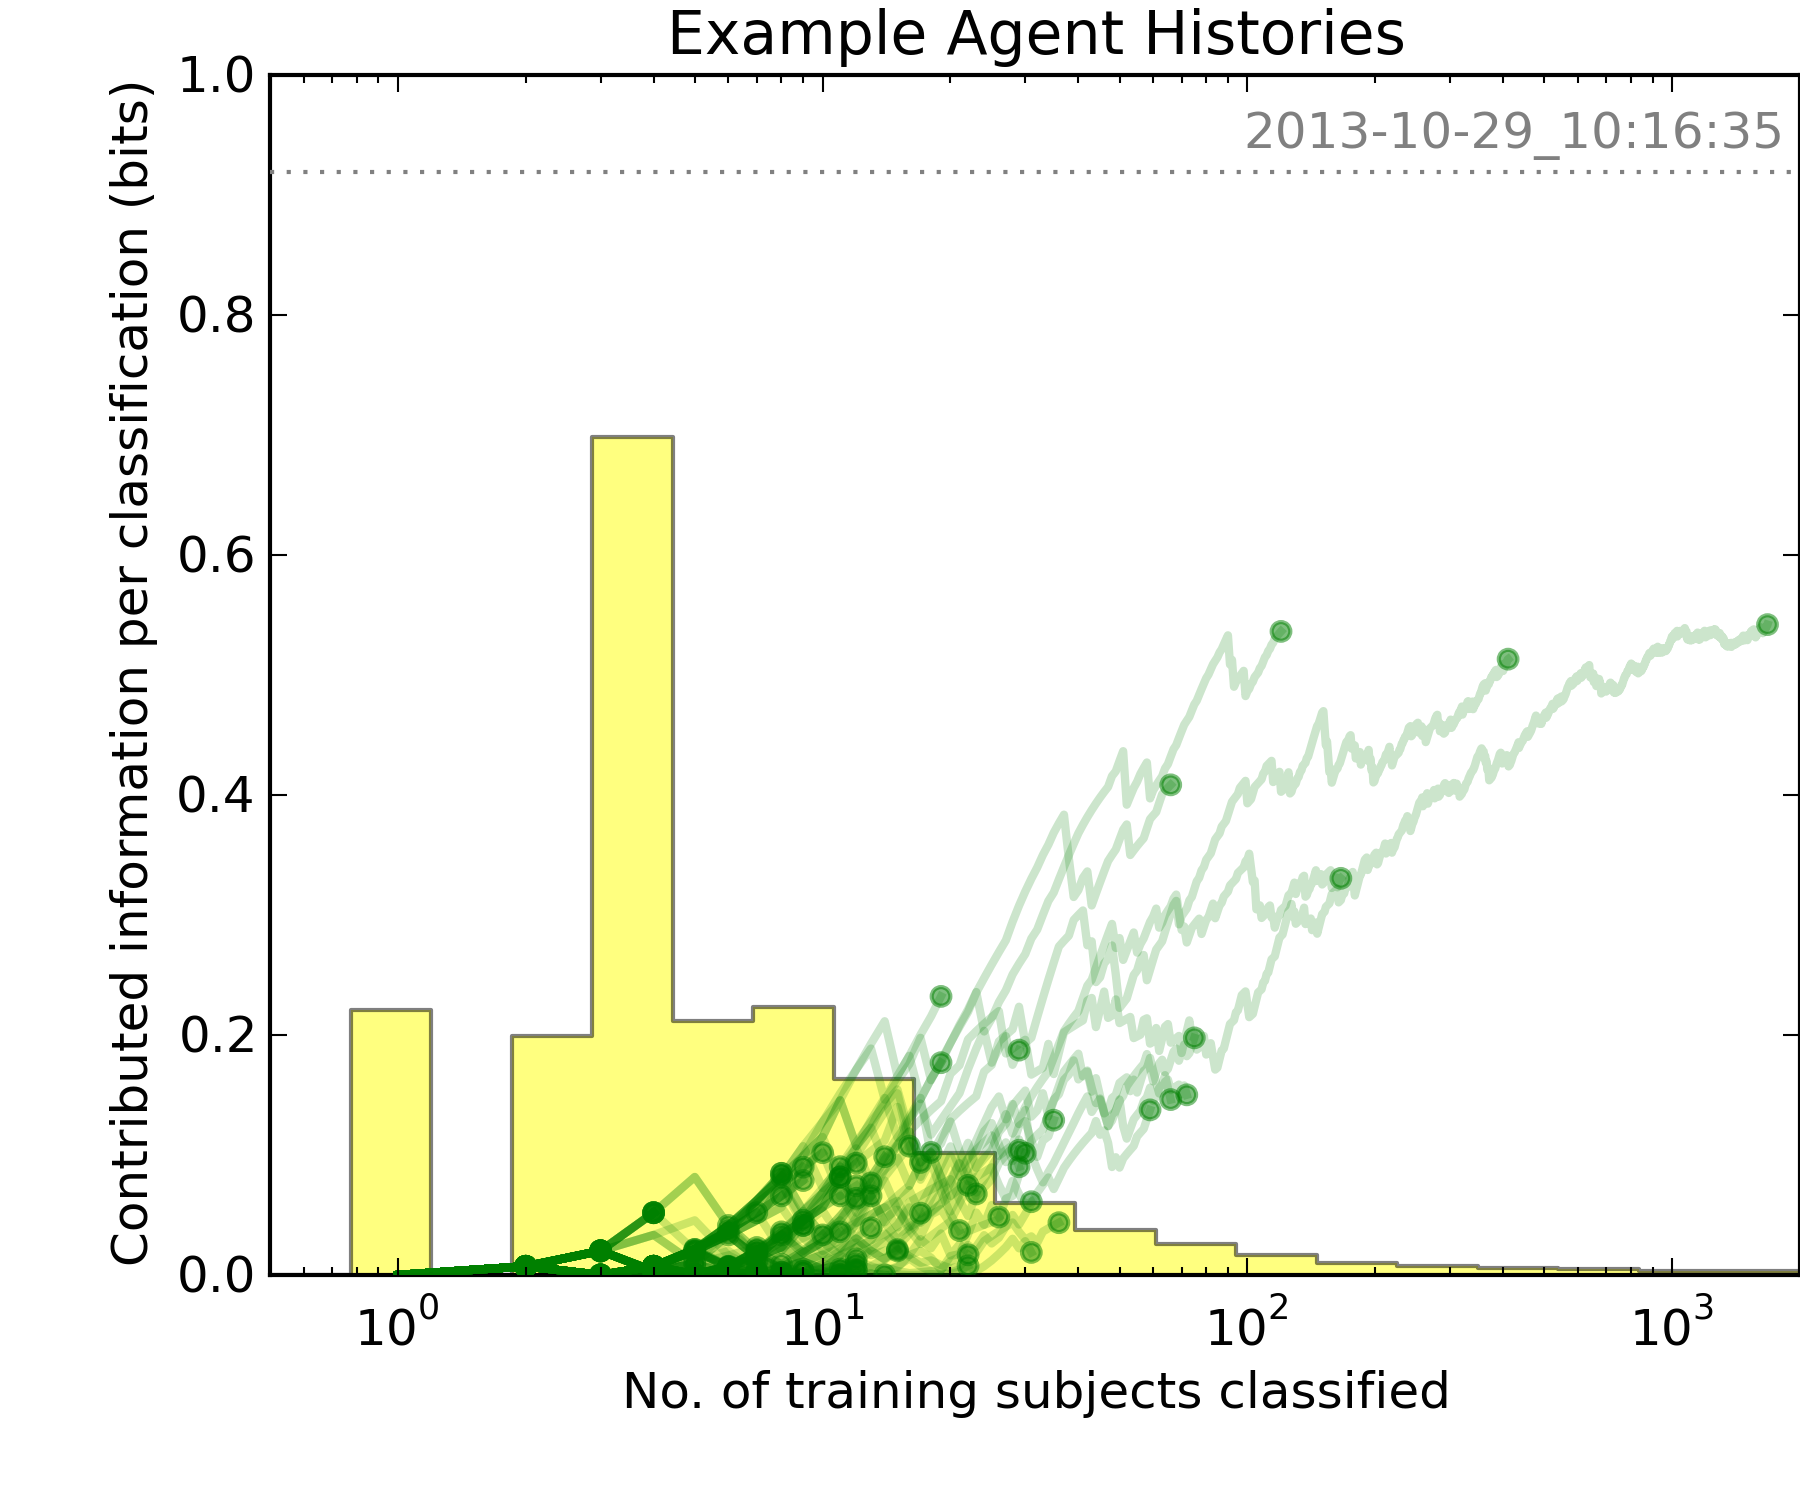
\includegraphics[width=0.9\linewidth]{sw-system-figs/CFHTLS_2013-10-29_10:16:35_histories.png}
\caption{Typical \SW Agent histories. The ``skill'' of the  same 200 random
Agents  as in \Fref{fig:swap:agent-probabilities} is plotted in green as a function
of the number  of subjects classified (``effort''). The yellow histogram in
the background shows the distribution of effort.}
\label{fig:swap:agent-histories}
\end{figure}
%%%%%%%%%%%%%%%%%%%%%%%%%%%%%%%%%%%%%%%

\Fref{fig:swap:agent-probabilities} shows a random selection of Agents'
confusion matrix elements, as they were on a particular day towards the end of
the CFHTLS project. Many volunteers classify  only a small number of images,
and so their Agents' confusion matrix elements remain close to their initial
values of (0.5,0.5). As more images are classified (shown by the yellow point
size), the Agents' matrix elements tend to move towards higher values, as the
volunteers attain greater skill levels (green point sizes, see
\Sref{sec:results} below) and the Agent learns more about them. In this
quadrant, the Agents perceive their volunteers to be ``astute.'' This trend is
more clearly seen in \Fref{fig:swap:agent-histories}, which shows the skill of
the same sample of Agents as the number of images classified increases. The
histogram shows the distribution of classification number: a long tail to very
high ``effort'' can be seen. 

In \Sref{sec:results} below, we define several quantities based on the 
probabilities listed above that serve to quantify the performance of the crowd
in terms of the information they provide via their classifications, and report
on the performance of the system in returning a sample of lens candidates
as a function of $\pr(\LENS|C,T)$ threshold.

%%%%%%%%%%%%%%%%%%%%%%%%%%%%%%%%%%%%%%%
\begin{figure}
\centering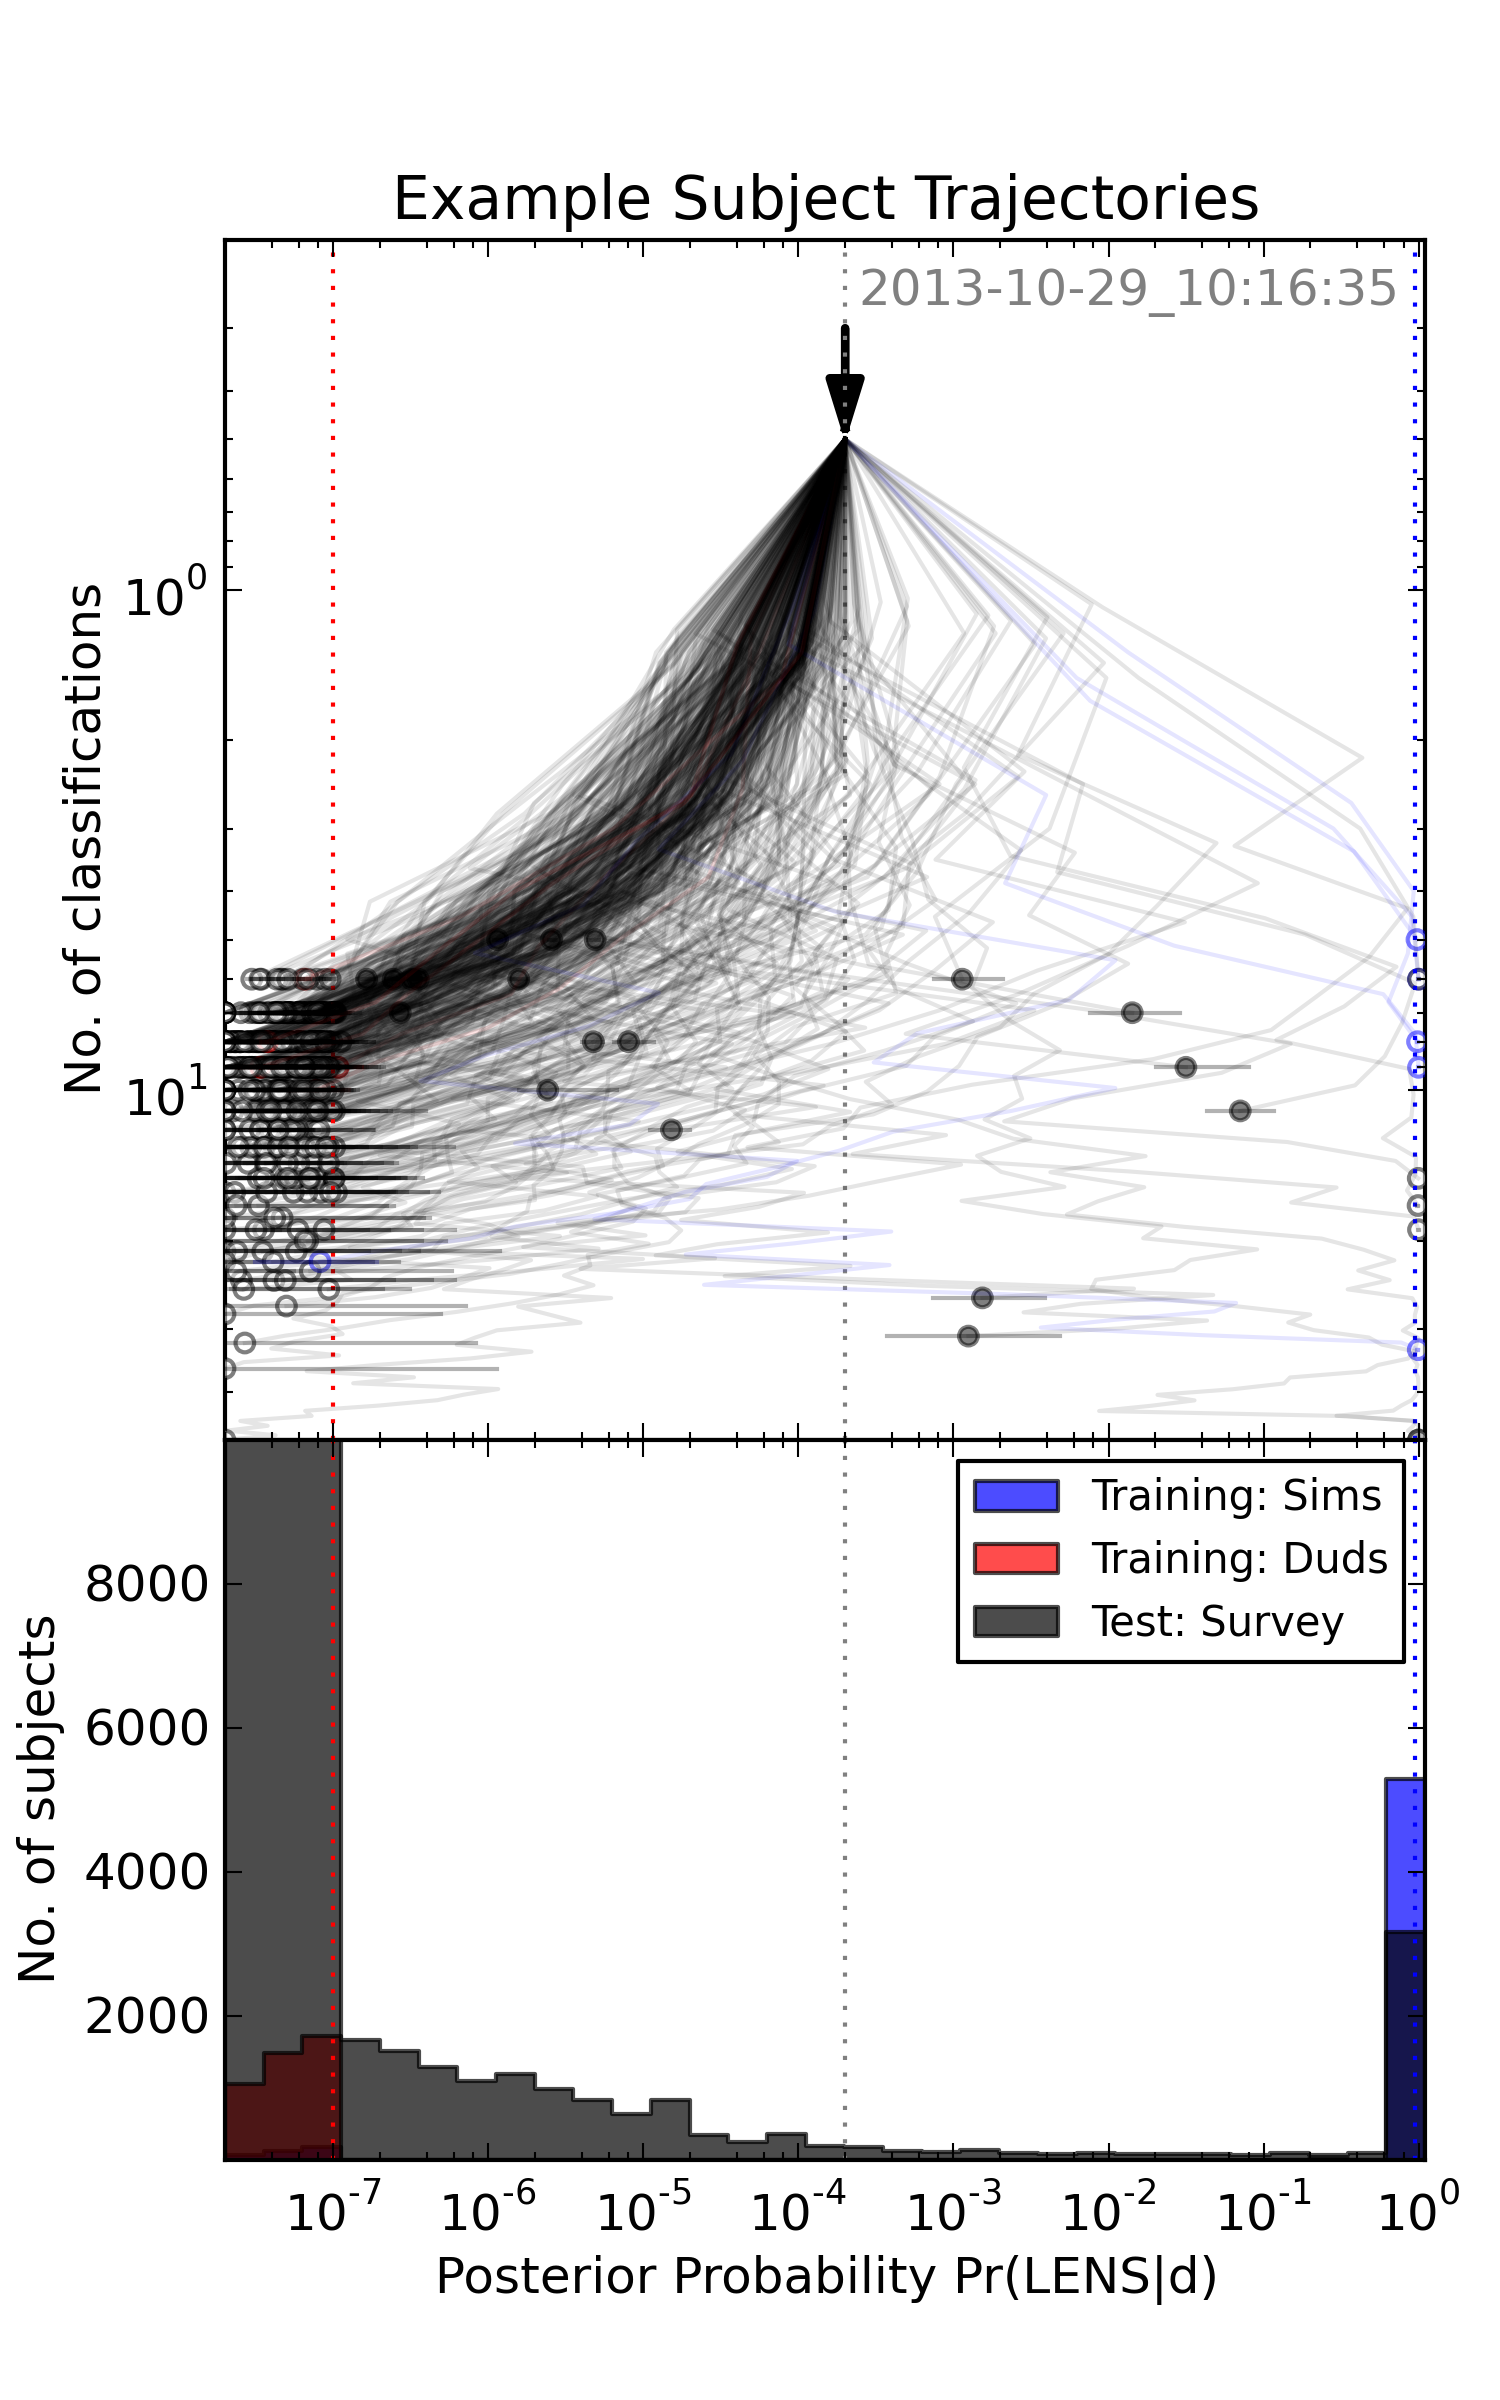
\includegraphics[width=0.9\linewidth]{sw-system-figs/CFHTLS_2013-10-29_10:16:35_trajectories.png}
\caption{Typical \SW stage 1 subject trajectories. Subjects drift downwards in
the top panel as they are classified, while being nudged left and right by the
Agents as they interpret the volunteers input. The dotted vertical lines show
(left to right) the retirement threshold, prior probability, and the detection
threshold.}
\label{fig:swap:subject-trajectories}
\end{figure}
%%%%%%%%%%%%%%%%%%%%%%%%%%%%%%%%%%%%%%%

During stage 1 classification of the CFHTLS images, we assigned a prior
probability for each image to contain a lens of $2\times10^{-4}$, based on a
rough estimate of the number of expected lenses in the survey. We then
assigned two values of the images' posterior probability, $\pr(\LENS|C,T)$, to
define ``detection'' and ``rejection'' thresholds. These were set to be 0.95
and (approximately symmetrically in the logarithm of probability), $10^{-7}$.
Subjects that attained probability of less than the rejection threshold were
scheduled for retirement and subsequently ignored by the analysis code.
Subjects crossing the detection threshold were not retired from the website,
but instead left in the system so that more volunteers could see them. The
progress of the subjects is illustrated in \Fref{fig:swap:subject-trajectories}.
Subjects appear on this plot at the tip of the arrow, at zero classifications
and prior probability; they then drift downwards as they are classified by the
crowd, with each Agent applying the appropriate kick in probability based on
what it hears its volunteer say. Encouragingly, sims (blue) tend to end up
with high probability, while duds (red) pile up at low probability; test
subjects (black) mostly drift to low probability, but some go the other way.
The latter will help make up the candidate sample. As this plot shows, around
10 classifications are required for a subject to reach the retirement
threshold.

The analysis code was run every night during the project, and subjects retired
in batches after its completion. This introduced some inefficiency, because
some classifications were accumulated in the time between them crossing the
rejection threshold and the subject actually being retired from the website.
As subjects were retired from the site, more subjects were activated. In this
way, the volunteers who down-voted images for not containing any lensed
features enabled new images to be shown to other members of the community.

When all the subjects had either been retired, or classified around 10 times
or more, the web app was paused and reconfigured for stage 2. The sample of
subjects classified during stage 2 was selected to be all those that passed
the detection threshold ($\pr(\LENS|C,T) > 0.95$) at stage 1. These were
classified for one week, with no retirement but a maximum classification
number of 50 each. 

\todo{Phil,Chris}{Write about offline analysis here (issue \#40)}


%%%%%%%%%%%%%%%%%%%%%%%%%%%%%%%%%%%%%%%%%%%%%%%%%%%%%%%%%%%%%%%%%%%%%%%%%%%%%%

\section{Results}
\label{sec:results}

In this section we present our findings about the performance of the  \sw
system, in terms of the information  contributed by the crowd in
\Sref{sec:results:crowd}, and the overall classifications of the training set
that they made. 

% % % % % % % % % % % % % % % % % % % % % % % % % % % % % % % % % % % % % % % 

\subsection{Crowd Properties}
\label{sec:results:crowd}


%%%%%%%%%%%%%%%%%%%%%%%%%%%%%%%%%%%%%%%
\begin{figure*}
\centering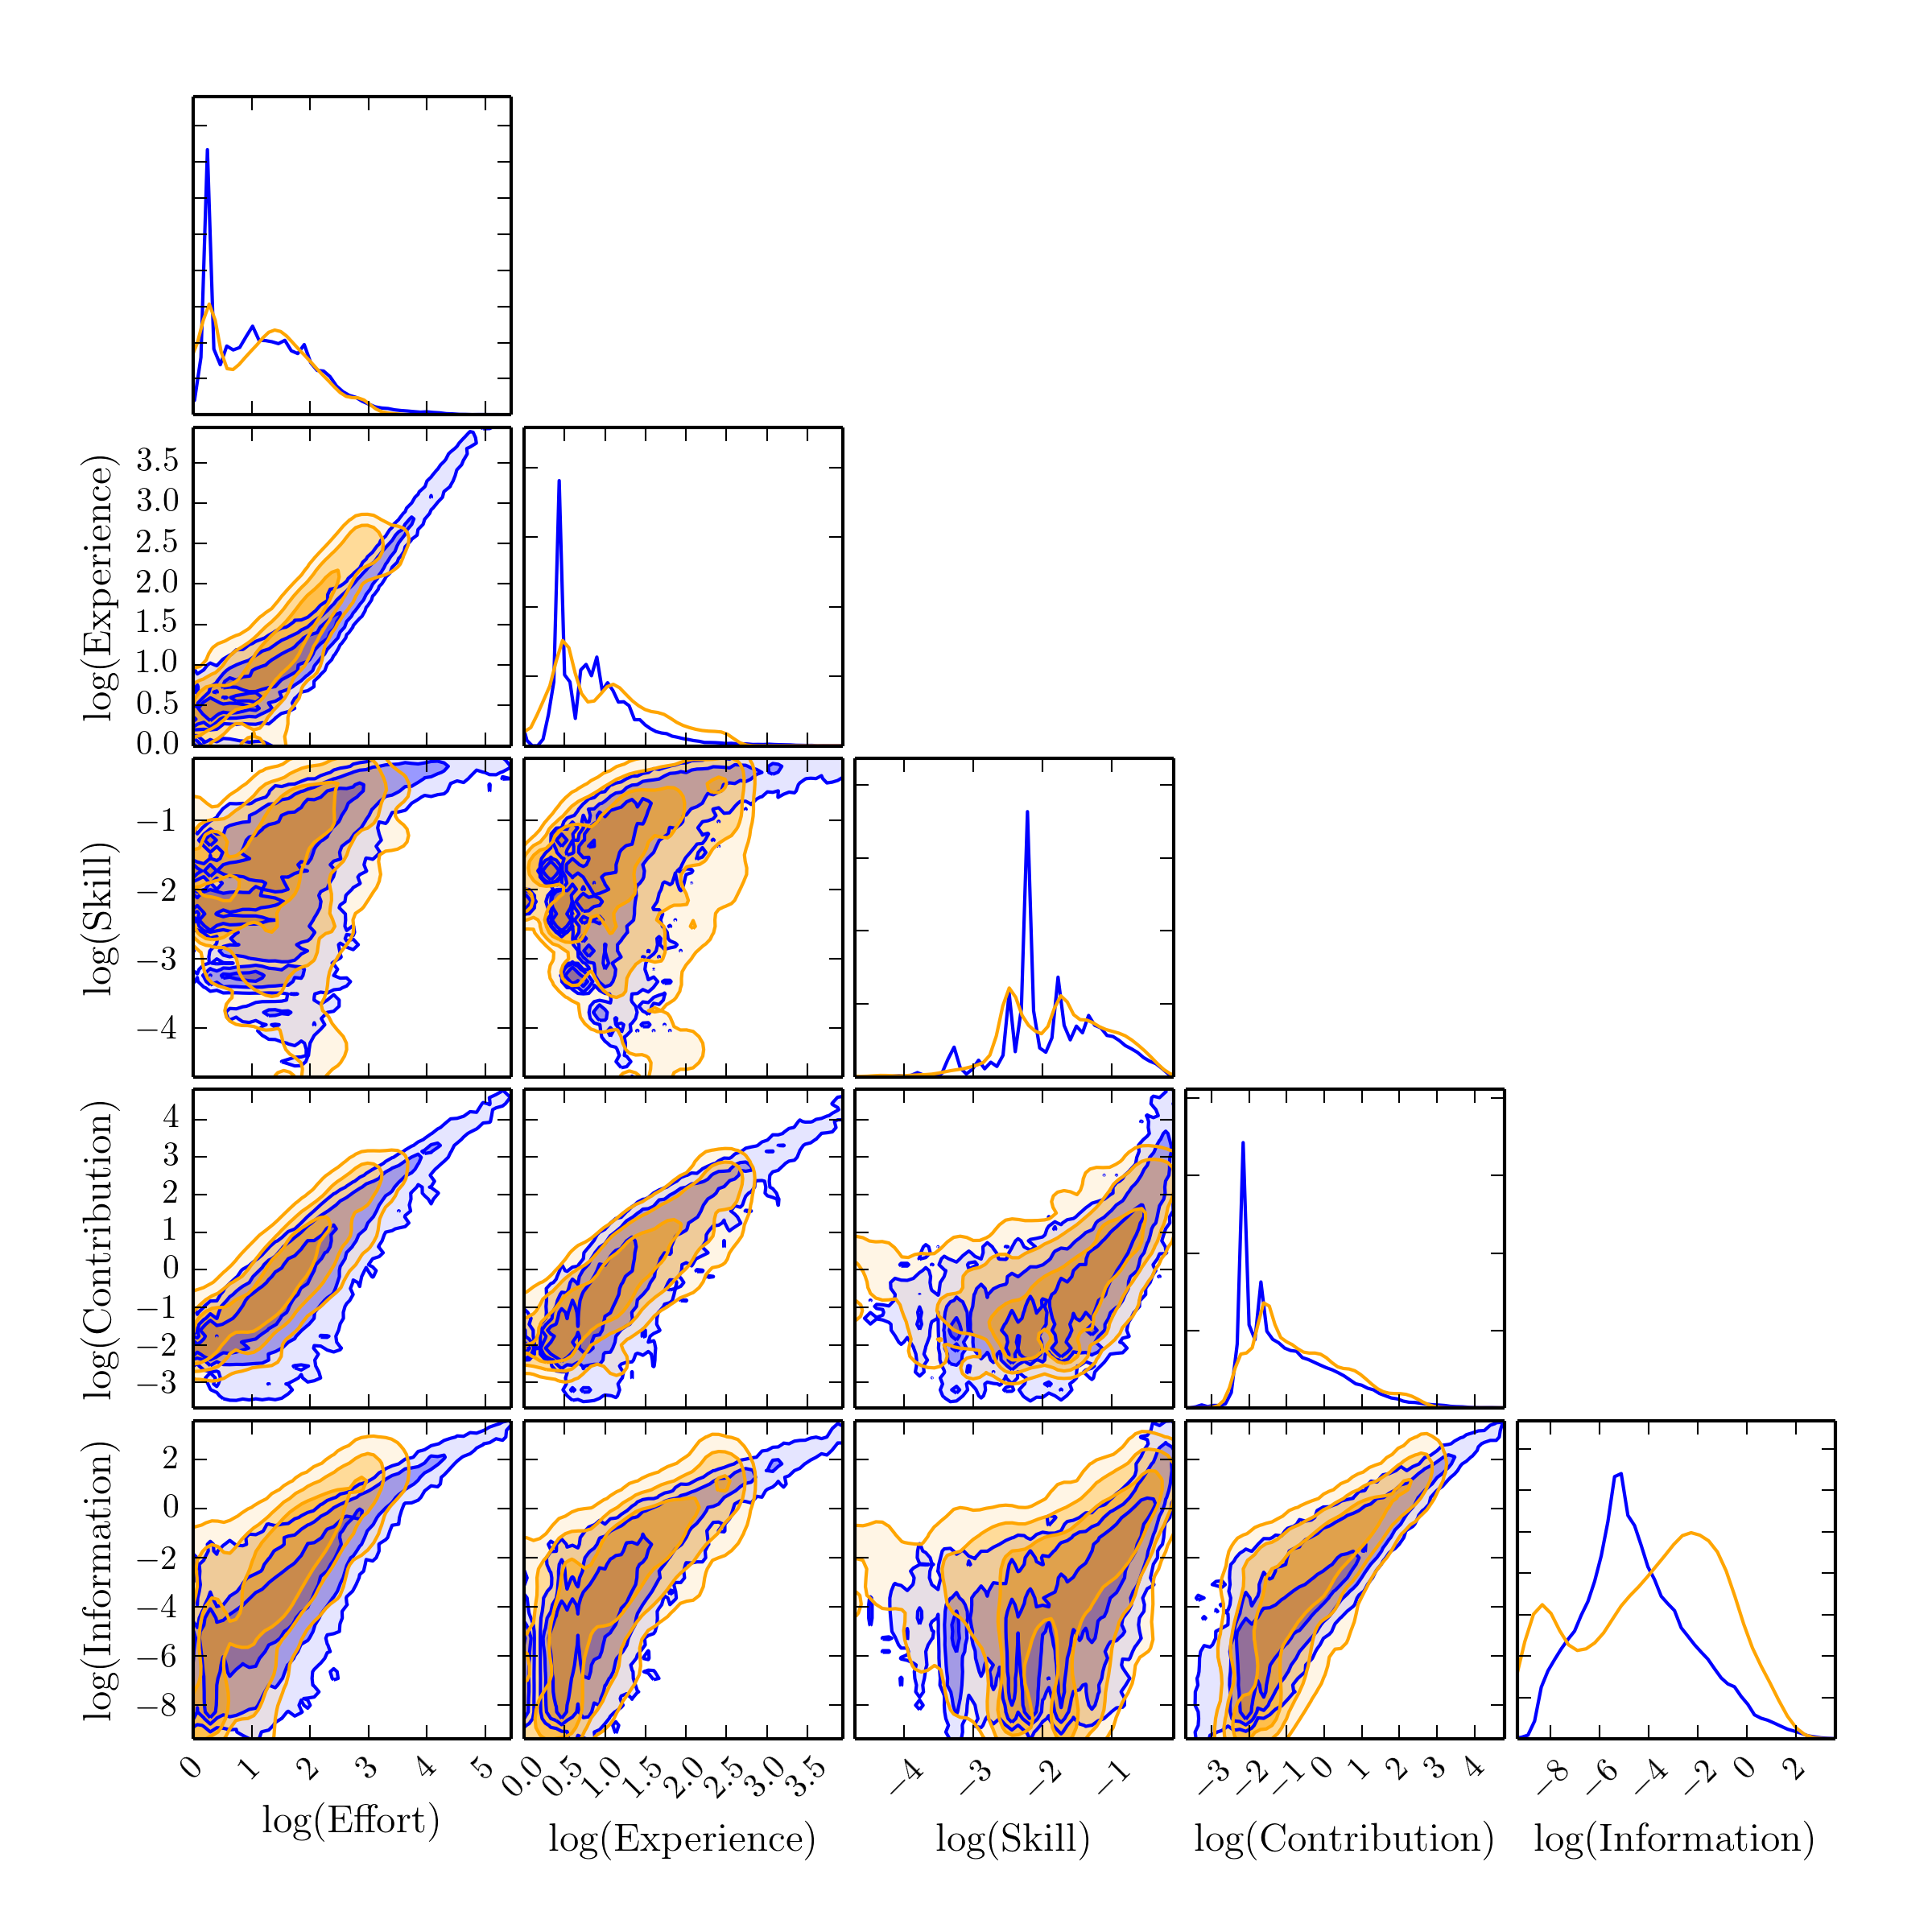
\includegraphics[width=0.9\linewidth]{sw-system-figs/all_skill_contribution_experience_education.png}
\caption{Key properties and contributions of the \sw crowd. Plotted are the
1-D and 2-D marginalized distributions for the logarithms of the 
properties of the agents described in the text. The stage 1 agents are shown
in blue, the stage 2 agents in orange.}
\label{fig:crowd:cornerplot}
\end{figure*}
%%%%%%%%%%%%%%%%%%%%%%%%%%%%%%%%%%%%%%%

We define the following properties of the crowd, as characterised by their
agents, and plot the distributions of their logarithms in
\Fref{fig:crowd:cornerplot}. 
%
\begin{description}
%
\item{\noindent\bf ``Effort:''} The number of test images, $\effort$, classified by a
volunteer. In stage 1, the mean effort per agent was 263; in the shorter stage
2 it was 81.
%
\item{\noindent\bf ``Experience:''} The number of training images, $\experience$,
classified by a volunteer. In stage 1, the mean experience per agent was 29;
in stage 2 (where the training image fequency was set higher) it was 34.
%
\item{\noindent\bf ``Skill:''} The expectation value of the information gain, 
$\skill$
should  the next subject classified have lens probability 0.5
(\Aref{appendix:swap}),  in bits. Random classifiers have $\skill = 0.0$,
perfect classifiers have $\skill = 1.0$. All agents start with $\skill = 0.0$;
this increases as training subjects are classified, and the agent's estimates
of its confusion matrix elements improve. In stage 1, the mean skill per agent
was 0.04 bits; in  stage 2 it was 0.05.
%
\item{\noindent\bf ``Contribution:''} The integrated skill over a volunteer's test
subject classification history, and represents the total  contribution to the
project that volunteer (see the appendix for more discussion of this
quantity). In stage 1, the mean contribution per agent was 34.9 bits; in 
stage 2 it was 33.5.
%
\item{\noindent\bf ``Information:''} The total information $\information$ generated by
the  agent during the volunteer's classification activity. This quantity
depends on the value of each subject's lens probability when that subject was 
presented to the volunteer (\Aref{appendix:swap}), and so there is an element
of luck involved with this quantity: if you never see a high probability
subject, it's hard to generate a large amount of information. You make your
own luck by classifying more subjects.
%
\end{description}

The leftmost column of \Fref{fig:crowd:cornerplot} shows how the last four of
these properties depends on the effort expended by the volunteers. We see that
experience is strongly correlated with effort (as training images are
presented throughout each stage, albeit at decreasing frequency), and that
this is also true for skill. In the second row of \Fref{fig:crowd:cornerplot}
we see that while skills of greater than 0.1 can be attained after just a few
training images, most agents of such low experience have significantly lower
skill. The volunteers in question only classify a few subjects before leaving.
However, at high values of experience and effort, the skill is \emph{always
high}. There seem to be very few agents logging large numbers of
classifications at low skill (although there are one or two exceptions): almost
all high effort ``super-users'' have high skill. These two properties are
reflected in both the contributions these volunteers make (third row) and the
information they generate (fourth row).

The distributions for the stage 2 agents (orange) are qualitatively similar to
those for the stage 1 agents (blue). Differences are: 1) the maximum effort
possible at stage 2 is smaller, because fewer subjects were available to be
classifed, but 2) the mean effort expended at stage 2 was higher (perhaps
because the subjects were higher probability, and more compelling); 3) the
information generated per agent was higher at stage 2, because the subjects
had higher probability.

%%%%%%%%%%%%%%%%%%%%%%%%%%%%%%%%%%%%%%%
\begin{figure}
\centering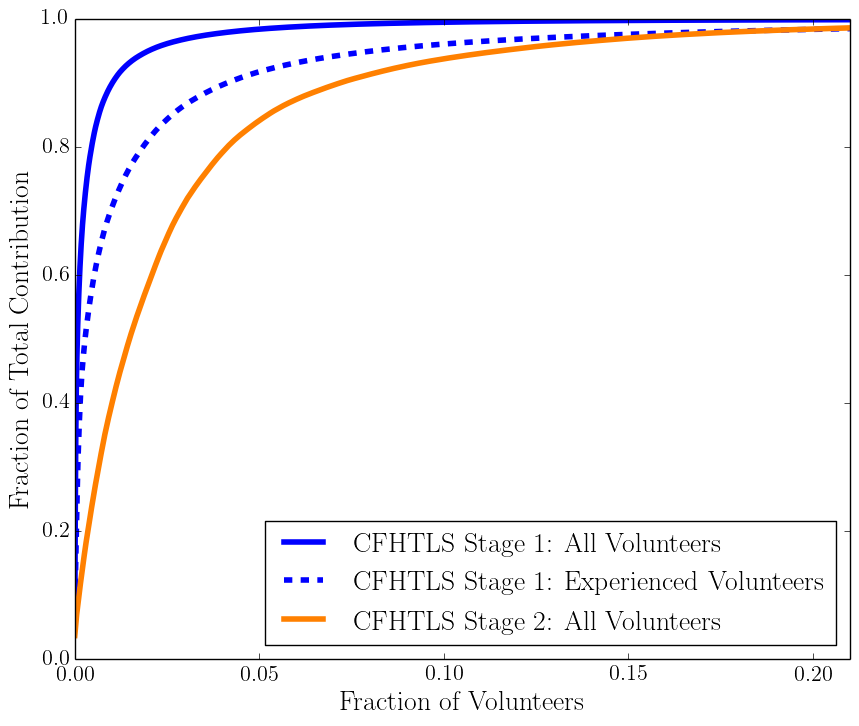
\includegraphics[width=0.9\linewidth]{sw-system-figs/crowd_contrib_cumul.png}
\caption{Narrow cumulative distributions of the contributions made by the
agents: for example, 90\% of the stage 2 contributions were made by the
highest contributing  7\% of the crowd. The stage 1 agents are shown in blue,
the stage 2 agents in orange. ``Experienced volunteers'' classified 10 or more
training subjects.}
\label{fig:crowd:cumulplot}
\end{figure}
%%%%%%%%%%%%%%%%%%%%%%%%%%%%%%%%%%%%%%%

\Fref{fig:crowd:cornerplot} shows the \sw crowd to have quite broad
distributions of logarithmic effort, skill, and contribution. To better
quantify the contributions made by the volunteers, we show their cumulative
distribution on a linear scale in \Fref{fig:crowd:cumulplot}. This plot shows
clearly the importance of the hardest-working, most active volunteers: at
stage 1,  1.0\% of the volunteers -- 375 people -- made 90\% of the
contribution.  At stage 2, where it was not possible to make as
many classifications before running out of subjects, 7.2\% of the volunteers
-- 141 people -- made 90\% of the contribution. 

However, it is not the case that only these small groups were capable of
making this large contribution: 9118 volunteers were ``experienced'' in that
they had all classified at least 10 training images; the 375 highest
contributing volunteers make up just 4\% of this experienced volunteer pool.
The cumulative distribution of agent skill is shown in
\Fref{fig:crowd:cumulskillplot}: these distributions are significantly broader
than the corresponding distributions of agent contribution in 
\Fref{fig:crowd:cumulplot}. The most skilled 20\% of agents possess only  79\%
of the skill at stage 1, and 77\% at stage 2. The inexperienced volunteers
also possess a significant fraction of the skill: the most skillful 20\% of
experienced volunteers (1824 people)  possess just 43\% of the total skill.
The level of contribution made at \sw by experienced volunteers is largely a
matter of choice (or perhaps, availability of time!).

%%%%%%%%%%%%%%%%%%%%%%%%%%%%%%%%%%%%%%%
\begin{figure}
\centering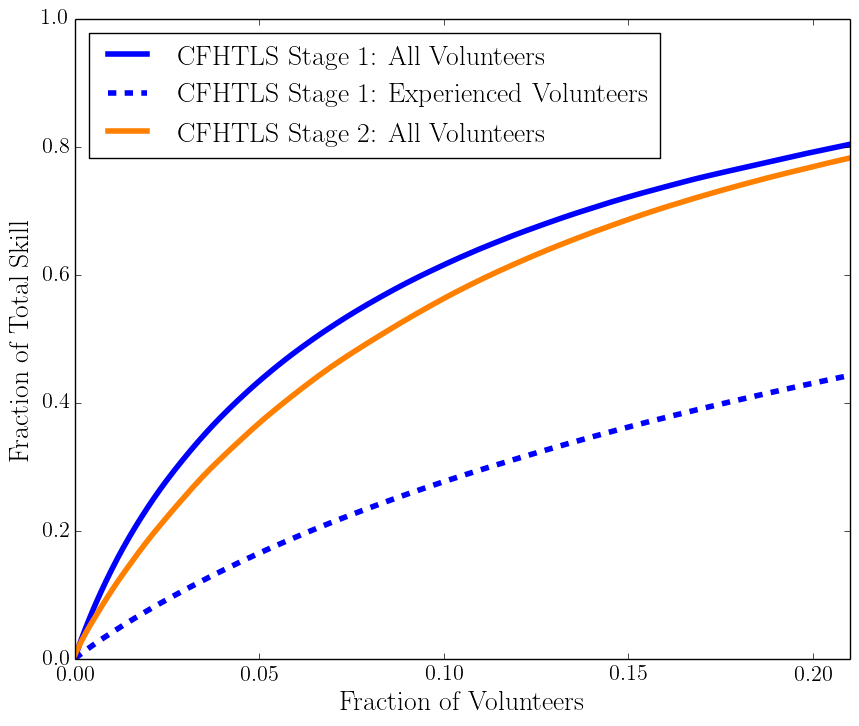
\includegraphics[width=0.9\linewidth]{sw-system-figs/crowd_skill_cumul.png}
\caption{Broad cumulative distributions of agent skill: 
the most skilled 20\% of the crowd only possess 79\% of the skill at stage 1.
The stage 1 agents
are shown in blue, the stage 2 agents in orange. ``Experienced volunteers''
classified 10 or more training subjects.}
\label{fig:crowd:cumulskillplot}
\end{figure}
%%%%%%%%%%%%%%%%%%%%%%%%%%%%%%%%%%%%%%%


%%%%%%%%%%%%%%%%%%%%%%%%%%%%%%%%%%%%%%%
\begin{figure}
\centering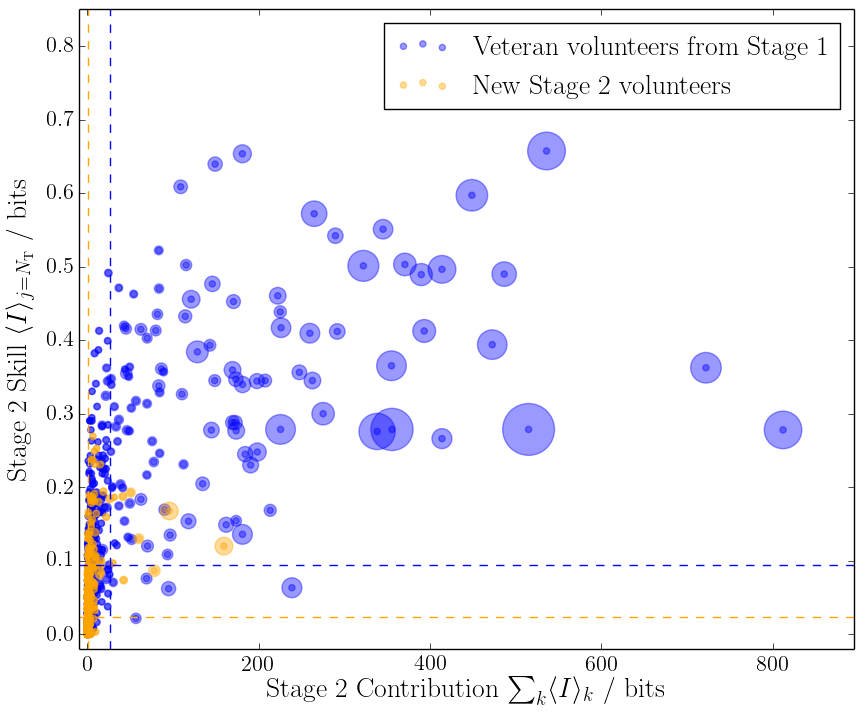
\includegraphics[width=0.9\linewidth]{sw-system-figs/stage2_veteran_contribution.png}
\caption{Stage 2 agent properties, separating veterans from stage 1 from new
volunteers. Point size represents total information generated, dashed lines
are drawn at the mean values for each sample.}
\label{fig:crowd:stage1vstage2}
\end{figure}
%%%%%%%%%%%%%%%%%%%%%%%%%%%%%%%%%%%%%%%

We now look at the transition between stage 1 and stage 2 in more detail. Of
the 1964 volunteers who took part in the stage 2 classification round, only
774 were veterans from stage 1. However, these volunteers showed significantly
higher skill levels than the new users, and also made more classifications
(and hence made greater contributions. This is illustrated in  
\Fref{fig:crowd:stage1vstage2}. In this figure, point size is proportional to
information generated: the higher skill, higher effort stage 1 veterans
generated most of the information.

%%%%%%%%%%%%%%%%%%%%%%%%%%%%%%%%%%%%%%%
\begin{figure}
\centering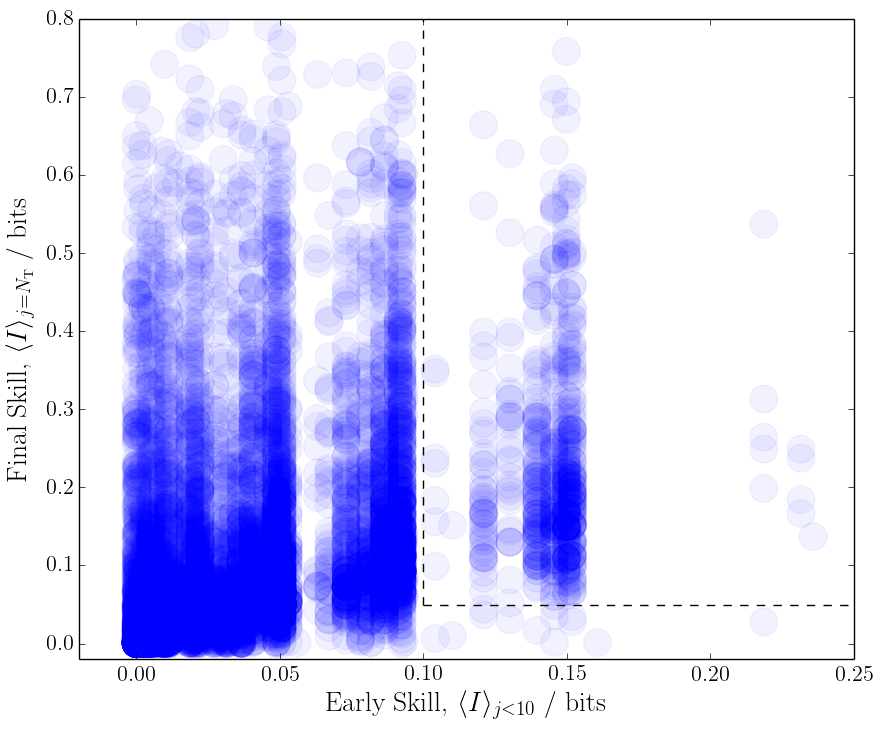
\includegraphics[width=0.9\linewidth]{sw-system-figs/early_vs_final_skill.png}
\caption{Predictability of final skill from early skill (after 10 training
classifications) in stage 1 agents. The dashed lines enclose 649 agents with
early skill greater than 0.1 
who retain final skill of greater than 0.05. Point size is proportional to
contribution (plus a constant).}
\label{fig:crowd:skillprediction}
\end{figure}
%%%%%%%%%%%%%%%%%%%%%%%%%%%%%%%%%%%%%%%

Having seen the importance of the high skill volunteers at both stage 1 and
stage 2, we might ask, can we predict agent skill after, say, the volunteer
has experienced 10 training subjects? In \Fref{fig:crowd:skillprediction} we
plot this ``early skill'' against final skill, for all experienced stage 1
volunteers. The majority of the crowd shows little correlation, but at the
high early skill end, some predictability appears. The 649 experienced  stage
1 volunteers who had early skill greater than 0.1 went on to attain a mean
final skill of 0.22, with 97\% remaining at skill 0.05 or higher. This
suggests that it might be worth tracking volunteers' skill as a project
progresses, in order to encourage those showing an aptitude for the task to
take part in the more difficult activities, such as stage 2 refinement.
However, this would not have done a very good job at identifying the 
volunteers who went on to make the largest contributions: the point size in 
\Fref{fig:crowd:skillprediction} is proportional to contribution (plus a constant):
many of the highest contributors showed relatively low skill early on.

\Tref{tab:crowd:contributions} shows the total effort, contribution, skill and
information generated in both stage 1 and 2 of the CFHTLS project, with the
total numbers of agents and subjects for comparison. These numbers allow us to
quantify the efficiency of the system. The contribution per classification is
defined in terms of a hypothetical subject with lens probability of 0.5; one
bit of information is needed to update such a subject's lens probability to
either zero or one. This means that a maximally complete classification stage
would yield a total contribution (summed over all agents) equal to the number
of subjects. The ratio of this hypothetical optimum to the actual total
contribution is therefore a measure of the stage's inefficiency. We find our
inefficiency (by dividing column 2 by column 3) to be 33\% and 17\% in stage 1
and 2 respectively. In stage 1, this inefficiency is due to the daily
processing: we were not able to retire subjects fast enough, and so they,
remained in the system, being over-classified. Only 3705745 classifications
were needed to retire all the subjects: the ratio of this to the total number
made is 34\%. (The remaining 1\% is due to not all subjects being classified
to 1 or 0 probability.) At stage 2, we did not retire any subjects at all; the
inefficiency in this case was by design, to give everyone a chance to
appreciate what they had found together! 

The total skill of the crowd, computed by summing the skill of all the agents,
is, similarly, a measure of the effective crowd size: a crowd of perfect
classifiers would be this size. The stage 1 crowd was equivalent to a team of
1469.9 perfect classifiers; the stage 2 crowd was equivalent to a team of
102.4 perfect classifiers. 

The total information generated during the survey is harder to interpret,
because it's exactly the high probability candidates that we leave in the
system that give rise to most of the information generated. What we can do is
divide the total information generated by the amount of information it takes
to classify a \sw subject all the way to the detection threshold (lens
probability 0.95), divide by this number, and then multiply by the survey
inefficiency to get a very rough estimate for the effective number of
detections corresponding to the crowd's contribution. With a prior probability
of $2\times10^{-4}$, it takes 12.3 bits to make a detection (see
\Sref{sec:appendix:infogain} in the appendix); the effective
number of detections contributed by the stage 1 and stage 2 volunteers is then
2830 and 25 bits respectively. 
These figures are close to the numbers of detections
given in column 7 of \Tref{tab:crowd:contributions}. 
The uncertainty in the interpretation of the
information generated provides further justification for our focus on the
expected information gain as a measure of volunteer contribution.

%%%%%%%%%%%%%%%%%%%%%%%%%%%%%%%%%%%%%%%
\begin{table*}
\begin{center}
\caption{Total crowd and subject sample properties from the CFHTLS project.}
\label{tab:crowd:contributions}
\begin{tabular}{cccccccc}
  \hline
  \hline {Stage} & Subjects & Contribution                          & Agents & Skill      & Classifications          & Candidates & Information \\
                 & $\Ns$    & $\sum_k^{\Nv} \contribution_k$ (bits) & $\Nv$  & $\sum_k^{\Nv} \skill_k$ (bits) & $\sum_k^{\Nv} \thiseffort$ & $\Ncands$  & $\sum_j^{\Ns}\sum_k^{\Nv} \information_{j,k}$ (bits) \\
  \hline 
            1    & $427064$ & $1292016.3$ & $36982$ & $1471.9$ & $10802125$ & $3368$ & $91122.6$ \\
            2    & $3679$   &   $21895.8$ &  $1964$ &  $102.4$ &   $224745$ &   $90$ &  $1640.4$ \\
  \hline \hline
\end{tabular}
\medskip\\
\end{center}
\end{table*}
%%%%%%%%%%%%%%%%%%%%%%%%%%%%%%%%%%%%%%%

% % % % % % % % % % % % % % % % % % % % % % % % % % % % % % % % % % % % % % % 

\subsection{Sample Properties}
\label{sec:results:sample}

We now quantify the performance of the \sw system in terms of the recovery of
the training set images. \Fref{fig:results:sample:roc} shows receiver
operating characteristic (ROC) curves for CFHTLS stage 1 and stage 2. These
plots show the true positive rate (TPR), the number of sims correctly detected
divided by the total number of sims in the training set, and the false
positive rate (FPR), the number of duds incorrectly detected  divided by total
number of duds in the training set, both for a given sample of detections defined by
a particular probability threshold, which varies along the curves.  In both
stages, these curves show that true positive rates of  around 90\% were
achieved, at very low false positive rates. For comparison we show the results
of an analysis where the classifications of  training images were ignored, and
none of the agents allowed to learn: they were instead assigned initial values
of their confusion matrices of 0.75 for each element, which then remained
constant. This emulates a very simple unweighted voting scheme, where all
classifications are treated equally. In this case, the TPR remains under 80\%
in stage 1 and 60\% in stage 2, showing the benefit of including training
images and allowing the agents to learn. The choice of initial confusion
matrix is not very important: the same 0.75 initial values applied to normal,
learning agents results in a slightly lower TPR than the default case,
indicating that initializing the system less conservatively results in
slightly worse performance.

The dot-dashed curves show the impact of the offline analysis. At stage 1 the
results are very similar to the online version that was actually run (solid
line), at stage 2 there seems to be some benefit to doing the analysis in this
way. Remarkably, over 85\% TPR is achieved at zero FPR. Alternatively, if one
is willing to accept a false positive rate of 5\%, the true positive rate
rises to over 95\%, showing that some of the sims that were missed in the
online analysis can be recovered by doing the analysis offline. The same is
true at stage 1, but to a much lower degree.

%%%%%%%%%%%%%%%%%%%%%%%%%%%%%%%%%%%%%%%
\begin{figure*}
\begin{minipage}{0.45\linewidth}
  \centering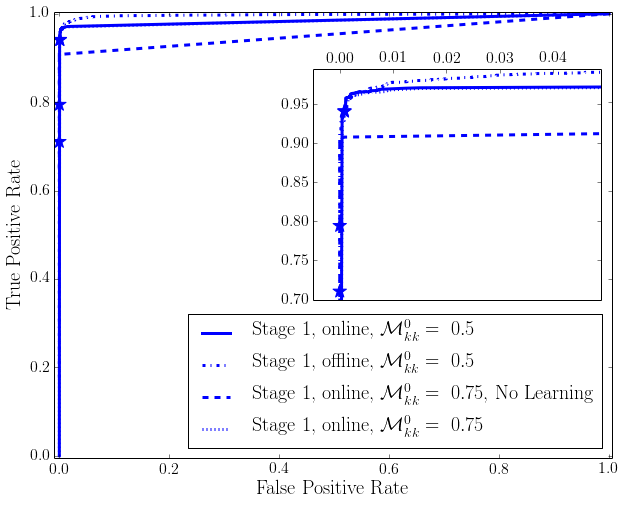
\includegraphics[width=\linewidth]{sw-system-figs/stage1_ROC.png}
\end{minipage}\hfill
\begin{minipage}{0.45\linewidth}
  \centering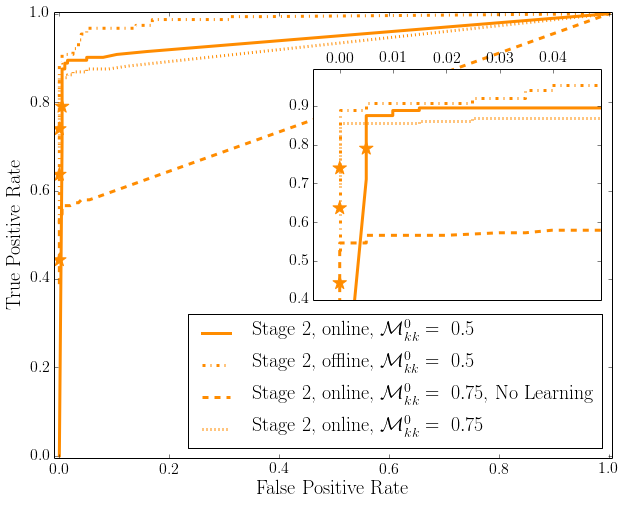
\includegraphics[width=\linewidth]{sw-system-figs/stage2_ROC.png}
\end{minipage}
\caption{Receiver operating characteristic curves for the \sw system, using
the CFHTLS training set. Left: stage 1, right: stage 2.}
\label{fig:results:sample:roc}
\end{figure*}
%%%%%%%%%%%%%%%%%%%%%%%%%%%%%%%%%%%%%%%

Adopting the online stage 1 analysis, and the offline stage 2 analysis, we
show in \Fref{fig:results:sample:CP} a plot of completeness versus purity in
the two stages. As in \Fref{fig:results:sample:roc}, the detection threshold
varies along the curves. Completeness is defined as the number of correctly 
detected sims divided by the total number of sims in the training set, while
purity is the number of the number of correctly detected sims divided by the
number of detections that would be claimed in a realistic sample. The purity
can only be calculated approximately. First we compute the expected number of
false positives by multiplying the FPR by the expected number of non-lenses in
the survey. Then we multiply the TPR by the expected number of lenses in the
survey, to get the expected number of true positives. The sum of the true
positives and the false positives gives the expected sample size; dividing the
expected number of true positives by this sample size gives the purity.


\todo{Chris}{Make completeness vs purity plot and add it here, please!}

%%%%%%%%%%%%%%%%%%%%%%%%%%%%%%%%%%%%%%%%%%%%%%%%%%%%%%%%%%%%%%%%%%%%%%%%%%%%%%

\section{Discussion}
\label{sec:discuss}

Challenges for future.

%%%%%%%%%%%%%%%%%%%%%%%%%%%%%%%%%%%%%%%%%%%%%%%%%%%%%%%%%%%%%%%%%%%%%%%%%%%%%%

\section{Conclusions}
\label{sec:conclude}

Summary of system.

Crowd-sourced gravitational lens detection works, in terms of the
classification of the training set as described here, in the following
specific ways: 

\begin{itemize} 

\item Participation (crowd size, activity rate) enabled project completion

\item Both stages (1 and 2) achieved the required rejection rates

\item Integrated humanpower = X (stage 1) and y (stage 2), cf hours taken by
small team of experts 

\item Nightly processing is inefficient: more classifications were made than
was necessary during peak participation. Need kafka...

\item Retirement rate. False negatives: which sims were missed?

\item The optimal true positive rate (completeness) and false positive rate in
the training set were estimated to be TPR\% and FPR\% at Stage 1, assuming a
detection threshold of xxx.  

\item In the ``refinement'' stage 2, X\% of the stage 1 candidates were
rejected (with P less than threshold), and the remainder assigned lens
``probabilities.'' Ranking
subjects by their Stage 2 lens probability gives an ROC curve for the system
with X properties. The optimal true positive rate (completeness) and false
positive rate in the training set were estimated as TPR\% and FPR\%; 

\item The lens-finding crowd shows some interesting properties, with
consequences for future scalability

\item The information comes predominantly from volunteers with agents with P =
...

\item The agents show a high mean information per classification, which
increased/decreased with time; this does/doesn?t correlate with active crowd
size, showing how the crowd changed over time...

\end{itemize}

Sum up, end.

%%%%%%%%%%%%%%%%%%%%%%%%%%%%%%%%%%%%%%%%%%%%%%%%%%%%%%%%%%%%%%%%%%%%%%%%%%%%%%
%%  ACKNOWLEDGMENTS
%%%%%%%%%%%%%%%%%%%%%%%%%%%%%%%%%%%%%%%%%%%%%%%%%%%%%%%%%%%%%%%%%%%%%%%%%%%%%%

\section*{Acknowledgements}
 
We thank all \Ncollaboration members of the \sw community for their
contributions to the project so far. A complete list of collaborators is
provided at \texttt{http://spacewarps.org/\#/results/CFHTLS}.

We are also grateful to Stuart Lynn, Kelly Borden, Laura Whyte, Brooke Simmons,
David Hogg, Thomas Jennings, Layne  Wright, Cecile Faure, Jonathan Coles, Stuart
Lowe and Jean-Paul Kneib for many useful conversations about citizen science and
gravitational lens detection, and to the Dark Energy Survey and Pan-STARRS strong
lensing science teams for their suggestions and encouragement.

PJM was given support by the Royal Society, in the form of a research
fellowship, and by the U.S. Department of Energy under contract number DE-AC02-76SF00515.
%
AV acknowledges support from the Leverhulme Trust in the form of a research
fellowship.
%
The work of AM and SM was supported by World Premier International Research
Center Initiative (WPI Initiative), MEXT, Japan. The work of AM was also supported in
part by National Science Foundation Grant No. PHYS-1066293 and the hospitality
of the Aspen Center for Physics.
%
% Zooniverse / Sloan Foundation.
%
% Other authors.
PJM and ES thank the Institute of Astronomy and Astrophysics, Academia Sinica
(ASIAA) and Taiwan's Ministry of Science and Technology (MOST) for their
financial support of the workshop ``Citizen Science in Astronomy'' in March
2014, at which some parts of the SWAP analysis was developed.

The \sw project is open source.
The web app was developed at \texttt{https://github.com/Zooniverse/Lens-Zoo}, and was supported by a grant from the Alfred P. Sloan Foundation, 
while the SWAP analysis software was developed at
\texttt{https://github.com/drphilmarshall/SpaceWarps}.

The CFHTLS data used in this work are based on observations obtained with
MegaPrime/MegaCam, a joint project of CFHT and CEA/IRFU, at the
Canada-France-Hawaii Telescope (CFHT) which is operated by the National Research
Council (NRC) of Canada, the Institut National des Science de l'Univers of the
Centre National de la Recherche Scientifique (CNRS) of France, and the
University of Hawaii. This work is based in part on data products produced at
Terapix available at the Canadian Astronomy Data Centre as part of the
Canada-France-Hawaii Telescope Legacy Survey, a collaborative project of NRC and
CNRS.


%%%%%%%%%%%%%%%%%%%%%%%%%%%%%%%%%%%%%%%%%%%%%%%%%%%%%%%%%%%%%%%%%%%%%%%%%%%%%%
%  APPENDICES
%%%%%%%%%%%%%%%%%%%%%%%%%%%%%%%%%%%%%%%%%%%%%%%%%%%%%%%%%%%%%%%%%%%%%%%%%%%%%%

\appendix

%%%%%%%%%%%%%%%%%%%%%%%%%%%%%%%%%%%%%%%%%%%%%%%%%%%%%%%%%%%%%%%%%%%%%%%%%%%%%%

\section{Probabilistic Classification Analysis}
\label{appendix:swap}

Our aim is to enable the construction of a sample of good lens candidates.
Since we aspire to making logical  decisions, we define a  ``good candidate''
as one which has a high posterior probability of being a lens, given the data:
$\pr(\LENS|\data)$. Our problem is to approximate this probability. The data~$\data$
in our case are the pixel values of a colour image. However, we can greatly
compress these complex, noisy sets of data by asking each volunteer what they
think about them. A complete  classification in \sw consists of a set of
Marker positions, or none at all. The null set encodes the statement from
the volunteer that the image in question is $\saidNOT$ a lens, while the
placement of any  Markers indicates that the volunteer considers this image to
contain a $\saidLENS$.  We simplify the problem by only using the Marker
positions to assess whether the volunteer  correctly assigned the
classification $\saidLENS$ or $\saidNOT$ after viewing (blindly) a member of
the training set of subjects. 

How should we model these compressed data? The circumstances of each
classification are quite complex, as are the human classifiers in general: the
volunteers learn more about the problem as they go, but also inevitably make
occasional mistakes (perhaps because a lens is difficult to see, or they
became distracted during the task). To cope with this uncertainty, we assign a
simple software {\it agent} to partner each volunteer. The agent's task is to
interpret their volunteer's classification data as best it can, using a model
that makes a number of necessary approximations. These interpretations will
then include uncertainty arising as a result of the volunteer's efforts and
also the agent's approximations, but they will have two important redeeming
features. First, the interpretations will be quantitative (where before they
were qualititative),  and thus will be useful in decision-making. Second, the
agent will be able to predict, using its model, the probability of a test
subject being a $\LENS$, given both its volunteer's classification, and its
volunteer's experience. In this appendix we describe how these agents work.


\subsection{Agents and their Confusion Matrices}
\label{appendix:swap:probabilities}

Each agent assumes that the probability of a volunteer recognising any given
simulated lens as a lens is some number, $\pr(\saidLENS|\LENS,\training)$, that
depends only on what the volunteer is currently looking at, and all the
previous training subjects they have seen (and not on what type of lens it is,
how faint it is, what time it is, \etc). Likewise, it also assumes that the
probability of a volunteer recognising any given dud image as a dud is some
other number, $\pr(\saidNOT|\NOT,\training)$, that also depends only on what the volunteer is currently looking at, and all the
previous training subjects they have seen. These two probabilities define a 
2 by 2 ``confusion matrix,'' which the agent updates, every time a
volunteer classifies a training subject, using the following 
very simple estimate:
\be
  \pr(``X"|X,\training) \approx \frac{N_{``X"}}{N_X}.
  \label{eq:app:fraction}
\ee
Here, $X$ stands for the true classification of the subject, \ie either
$\LENS$ or $\NOT$, while $``X''$ is the corresponding classification
made by the volunteer on viewing the subject. $N_X$ is the number of
lenses the volunteer has been shown, while $N_{``X"}$ is the number of 
times the volunteer got their classifications of this type of training subject
right. $\training$ stands for all
$N_{\LENS} + N_{\NOT}$ training data that the agent has heard about to
date. 

The full confusion matrix of the $k^{\rm th}$ volunteer's agent is therefore:
\begin{align}
  \CM^k &= 
  \begin{bmatrix}
    \pr(\saidLENS|\NOT,\trainingk) & \pr(\saidLENS|\LENS,\trainingk) \\
    \pr(\saidNOT |\NOT,\trainingk) & \pr(\saidNOT |\LENS,\trainingk)
  \end{bmatrix}, \notag \\
        &=
  \begin{bmatrix}
    \CM_{LN} & \CM_{LL} \\
    \CM_{NN} & \CM_{NL}
  \end{bmatrix}^k.
  \label{eq:confmat}
\end{align}
Note that these probabilities are normalized, such that
$\pr(\saidNOT |\NOT) = 1 - \pr(\saidLENS|\NOT)$.

Now, when this volunteer views a test subject, 
it is this confusion matrix that will allow their agent to update the
probability of that test subject being a $\LENS$. Let us suppose that
this subject has never been seen before: the agent assigns a 
prior probability that it is (or contains) a lens is 
\be
  \pr(\LENS) = p_0
\ee
where we have to assign a value for $p_0$. In the CFHTLS, we might expect
something like 100 lenses in 430,000 images, so $p_0 = 2\times10^{-4}$
is a reasonable estimate. The volunteer then makes a classification $C_k$ 
($= \saidLENS$ or $\saidNOT$).
We can apply Bayes' Theorem to derive how the agent should
update this prior probability into a posterior one using this new information:
\begin{align}
  \label{eq:app:first}
  & \pr(\LENS|C_k,\trainingk) = \\
  & \frac{\pr(C_k|\LENS,\trainingk)\cdot\pr(\LENS)}
{\left[ \pr(C_k|\LENS,\trainingk)\cdot\pr(\LENS) + \pr(C_k|\NOT,\trainingk)\cdot\pr(\NOT) \right]},
  \notag
\end{align}
which can be evaluated numerically using the elements of the confusion
matrix. 

\subsection{Examples}
\label{appendix:swap:examples}

Suppose we have a volunteer who is always right about the true
nature of a training subject. 
Their agent's confusion matrix would be
\be
  \CM^{\rm perfect} = 
  \begin{bmatrix}
    0.0 & 1.0 \\
    1.0 & 0.0
  \end{bmatrix}.
\ee
On being given a fresh subject that actually is a $\LENS$, this hypothetical
volunteer would submit $C = \saidLENS$.  Their agent would then calculate the
posterior probability for the subject being a $LENS$ to be
\begin{align}
  \pr(\LENS|\saidLENS,\trainingk) &= \frac{1.0 \cdot p_0}
           {\left[ 1.0\cdot p_0 + 0.0\cdot(1 - p_0) \right]}
   &= 1.0,
\end{align}
as we might expect for such a {\it perfect} classifier.  Meanwhile, a
hypothetical volunteer who (for some reason) wilfully always submits the wrong
classification would have an agent with the column-swapped confusion matrix
\be
  \CM^{\rm obtuse} = 
  \begin{bmatrix}
    1.0 & 0.0 \\
    0.0 & 1.0
  \end{bmatrix},
\ee
and would submit $C = \saidNOT$ for this subject. However, such a volunteer
would nevertheless be submitting useful information, since given the above
confusion matrix, their agent would calculate
\begin{align}
  \pr(\LENS|\saidNOT,T_k) &= \frac{1.0 \cdot p_0}
           {\left[ 1.0\cdot p_0 + 0.0\cdot(1 - p_0) \right]}
   &= 1.0.
\end{align}
{\it Obtuse} classifiers turn out to be as helpful as {\it perfect} ones.


\subsection{Updating the Subject Probabilities}
\label{appendix:swap:examples}

Suppose the $k+1^{\rm th}$ volunteer now submits a classification, on the same
subject just classified by the $k^{\rm th}$ volunteer. We can generalise
\Eref{eq:app:first} by replacing the prior probability with the current
posterior probability:
\begin{align}
  \label{eq:app:update}
  \pr(\LENS & |C_{k+1},\training_{k+1},\data) = \\
  & \frac{1}{Z} \pr(C_{k+1}|\LENS,\training_{k+1}) \cdot \pr(\LENS|\data) \\ \notag
{\rm where}\;\; Z = & \pr(C_{k+1}|\LENS,\training_{k+1})\cdot\pr(\LENS|\data) \\ \notag
      & + \pr(C_{k+1}|\NOT,\training_{k+1})\cdot\pr(\NOT|\data), \notag
\end{align}
and $\data = \{C_k,\trainingk\}$ is the set of all previous
classifications, and the set of training subjects seen by each of those
volunteers.
$\pr(\LENS|\data)$ is the fundamental property of each test subject that
we are trying to infer. We track $\pr(\LENS|\data)$ as a function of time,
and by comparing it to a lower or upper thresholds, make decisions about
whether to retire the subject from the classification interface or
promote it in \Talk, respectively.


\subsection{Information Gain per Classification, Agent ``Skill'' and ``Contribution''}
\label{appendix:swap:examples}

With an agent's confusion matrix in hand we can compute the
\emph{information} generated in any given classification. This will
depend on the confusion matrix elements (\Eref{eq:confmat}) but also on
the probability of the subject being classified containing a lens. The
quantity of interest is the relative entropy, or Kullback-Leiber
divergence, between the prior and
posterior probabilities for the possible truths $T$
given the submitted classification $C$:
\begin{align}
\information =& \sum_T \pr(T|C) \log_2 \frac{\pr(T|C)}{\pr(T)}     \notag \\
             =&    \pr(\LENS|C) \log_2 \frac{\pr(C|\LENS)}{\pr(C)} \notag \\
             +&    \pr(\NOT|C)  \log_2 \frac{\pr(C|\NOT)}{\pr(C)},
\end{align}
where, as above, $C$ can take the values $\saidLENS$ or $\saidNOT$. 
Substituting for the posterior probabilities using \Eref{eq:app:first} we get
an expression that just depends on the elements of the 
confusion matrix $\CM$ and the pre-classification subject lens
probability $\pr(\LENS) = p$:
\begin{align}
\information =    &     p \frac{\CM_{CL}}{p_c} \log_2 \frac{\CM_{CL}}{p_c}  \notag \\
                  & +(1-p)\frac{\CM_{CN}}{p_c} \log_2 \frac{\CM_{CN}}{p_c},
  \label{eq:app:infogain}
\end{align}
where the common denominator $p_c = p\CM_{CL} + (1-p)\CM_{CN}$. This
expression has many interesting features.  If $p$ is either zero or one,
$\information(C) = 0$  regardless of the value of $C$ or the values of
the confusion matrix elements: if we know the subject's status with
certainty, additional classifications supply no new information. If we
set $p$ to be the prior probability, \Eref{eq:app:infogain} tells us how
much information is generated by classifying it all the way to $p = 1$
(which a perfect classifier, with $\CM_{LL} = \CM_{NN} = 1$, can do in a
single classification). For a prior probability of $2\times 10^{-4}$, 
12.3 bits are generated in such a ``detection.''  Conversely, only
0.0003 bits are generated during the rejection of a subject with the
same prior: we are already fairly sure that each subject does not
contain a lens! Imperfect classifiers (with $\CM_{LL}$ and $\CM_{NN}$
both less than 1)  generate less than these maximum amounts of
information each classification; the only classifiers that generate zero
information are those that have $\CM_{LL} = 1 - \CM_{NN}$ (or
equivalently, $\CM_{CL} = \CM_{CN}$ for all values of $C$). We might
label such classifiers as ``random'', since they are as likely to
classify a subject as a $\saidLENS$ no matter the true content of that
subject. 

\Eref{eq:app:infogain} suggests a useful information theoretical 
definition of the classifier skill  perceived by the agent. At a fixed
value of $p$, we can take the expectation value of the information gain
$\information$ over  the possible classifications that could be made:
\begin{align}
\langle\information\rangle   =& \sum_C \sum_T \pr(T|C) \pr(C) \log_2 \frac{\pr(T|C)}{\pr(T)} \notag \\ 
         =& - \sum_T \pr(T) \log_2 \pr(T) \notag \\ 
          & + \sum_C \pr(C) \sum_T \pr(T|C) \log_2 \pr(T|C) \notag \\ 
         =&         p  \left[ \mathcal{S}(\CM_{LL}) + \mathcal{S}(1-\CM_{LL}) \right] \notag \\
          &     +(1-p) \left[ \mathcal{S}(\CM_{NN}) + \mathcal{S}(1-\CM_{NN}) \right] \notag \\
          & - \mathcal{S}\left[ p    \CM_{LL}       + (1-p)(1-\CM_{NN})     \right] \notag \\
          & - \mathcal{S}\left[ p (1-\CM_{LL})      + (1-p)   \CM_{NN}      \right] 
\end{align}
where $\mathcal{S}(x) = x \log_2{x}$. If we choose to
evaluate $\langle\information\rangle$ at $p = 0.5$, the result has some
useful properties. While random classifiers presented with  $p = 0.5$
subjects have $\skill = 0.0$  as expected, perfect classifiers appear to
the agents to have  $\skill = 1.0$. This suggests that  $\skill$, the
amount of information we expect to  gain when a classifier is presented
with a 50-50 subject, is a reasonable quantification of 
\emph{normalised skill}. A consequence of this choice is that the
integrated skill (over all agents' histories) should come out to be
approximately 
equal to the number of subjects in the survey, when the search is
``complete'' (and all subjects are fully classified). Therefore, a
particular agent's integrated skill is a reasonable 
measure of that classifier's
\emph{contribution} to the lens search.

We conservatively initialize both elements of each  agent's confusion
matrix to be $\CM^0_{LL} = \CM^0_{NN} = 0.5$, that of a maximally ambivalent  random classifier, so
that all agents start with zero skill. While  this makes no allowance
for volunteers that actually do have previous experience of what
gravitational lenses look like, we might expect it to help mitigate
against false positives. Anyone who classifies more than one image (by
progressing beyond the tutorial) makes a non-zero information
contribution to the project.


\subsection{Uncertainty in the Agent Confusion Matrices}
\label{appendix:swap:uncertainty}

Finally, the confusion matrix obtained from the application of
\Eref{eq:app:fraction} has some inherent noise which reduces as the
number of training subjects classified by the agent's volunteer
increases. For simplicity, the discussion has thus far assumed the case
when the confusion matrix is known perfectly; in practice, we allow for
uncertainty in the agent confusion matrices by averaging over a small
number of samples drawn from Binomial distributions characterised by the
matrix elements $\pr(C_k|\LENS,\trainingk)$ and  $\pr(C_k|\NOT,\trainingk)$. The
associated standard deviation in the estimated subject probability
provides an error bar for this quantity.

% For ease of notation, we will denote $\pr(C_k|\LENS,T_k)\equiv p_L$ and
% $\pr(C_k|\NOT,T_k)\equiv p_N$. In reality, there is a probability distribution
% for both $p_L$ and $p_N$. Let $p_0$ be the prior probability of the subject
% being a lens. Then the posterior probability, $p_0'$ of the subject being a
% lens after the classification $C_k$ is
% \be
%   \label{eq:app:sec}
% p_0' = \frac{p_L p_0}{\left[ p_L p_0 + p_N (1- p_0) \right]},
% \ee
% The posterior probability distribution $p_0'$ can be obtained by marginalizing
% over the probability distributions of $p_L$, $p_N$ and the prior probability
% distribution $p_0$ such that,
% \be
% P(p_0') = \int p_0' P(p_L) P(p_N) P(p_0) dp_L dp_N dp_0\,.
% \ee
% This marginalization is not analytically tractable. Therefore, we have
% implemented the following Monte-Carlo solution for this problem.
% 

%Finally, we also need to update the confusion matrix of an agent and obtain the
%variance on each element of the matrix, once a training subject has been
%classified. We would like to derive the posterior probability of the
%probability elements $p_1$ and $p_2$ given their prior probabilities. For this
%purpose, we can again make use of Bayes' theorem,
%\begin{equation}
%P(p_x'|N_{"X"},N_X,T) = \frac{P(N_{``X"}|p_x',N_X,T) P(p_x'|N_X,T)}{\sum_{N_{``X"}} P(N_{``X"}|p_x',N_X,T) P(p_x'|N_X,T)}
%\end{equation}
%Here, $P(N_{``X"}|p_x',N_X,T)$ is a binomial distribution, although this is not
%true strictly speaking given that our agents are learning and the values of the
%confusion matrix are moving. Modelling the learning curve of our users is yet
%another complicated extension we could think about.


\todo{Phil,Chris}{Write about offline analysis here (issue \#40)}


%%%%%%%%%%%%%%%%%%%%%%%%%%%%%%%%%%%%%%%%%%%%%%%%%%%%%%%%%%%%%%%%%%%%%%%%%%%%%%
%  REFERENCES
%%%%%%%%%%%%%%%%%%%%%%%%%%%%%%%%%%%%%%%%%%%%%%%%%%%%%%%%%%%%%%%%%%%%%%%%%%%%%%

% MNRAS does not use bibtex, input .bbl file instead. 
% Generate this in the makefile using bubble script in scriptutils:

% bubble -f paper-lcr.tex references.bib 
% \input{paper-lcr.bbl}

\bibliographystyle{apj}
\bibliography{references}


%%%%%%%%%%%%%%%%%%%%%%%%%%%%%%%%%%%%%%%%%%%%%%%%%%%%%%%%%%%%%%%%%%%%%%%%%%%%%%

\label{lastpage}
\bsp

\end{document}

%%%%%%%%%%%%%%%%%%%%%%%%%%%%%%%%%%%%%%%%%%%%%%%%%%%%%%%%%%%%%%%%%%%%%%%%%%%%%%
